\documentclass[a4paper,10pt]{article}
\usepackage[utf8]{inputenc}

% ----  Useful packages % ---- 
\usepackage{amsmath}
\usepackage{graphicx}
\graphicspath{{images/}}
\usepackage{amsfonts}
\usepackage{amsthm}
\usepackage{amssymb}
\usepackage{makecell}
\usepackage{mathtools}
\usepackage{tikz}
\usepackage{pgfplots}
\usepackage{float}
\usetikzlibrary{arrows.meta}

% ----  Useful packages % ---- 

\usepackage{wrapfig}
\usepackage{caption}
\usepackage{subcaption}
\usepackage{hyperref}
\hypersetup{
	colorlinks,
	citecolor=black,
	filecolor=black,
	linkcolor=black,
	urlcolor=black
}

% ---- Set page size and margins replace ------
\usepackage[letterpaper,top=2cm,bottom=2cm,left=3cm,right=3cm,marginparwidth=1.75cm]{geometry}
% ---- Set page size and margins replace ------

% ------- NOTA ------
\theoremstyle{remark}
\newtheorem{note}{Note}[subsection]
% ------- NOTA ------

% ------- OSSERVAZIONE ------
\theoremstyle{definition}
\newtheorem{observation}{Osservazione}[subsection]
% ------- OSSERVAZIONE ------

% ------- DEFINIZIONE ------
\theoremstyle{plain}
\newtheorem{definition}{Definizione}[subsection]
% ------- DEFINIZIONE ------

% ------- ESEMPIO ------
\theoremstyle{definition}
\newtheorem{example}{Esempio}[subsection]
% ------- ESEMPIO ------

% ------- DIMOSTRAZIONE ------
\theoremstyle{definition}
\newtheorem{demostration}{Dimotrazione}[subsection]
% ------- DIMOSTRAZIONE ------

% ------- TEOREMA ------
\theoremstyle{definition}
\newtheorem{theorem}{Teorema}[subsection]
% ------- TEOREMA ------

% ------- COROLLARIO ------
\theoremstyle{plain}
\newtheorem{corollaries}{Corollario}[theorem]
% ------- COROLLARIO ------

% ------- PROPOSIZIONE ------
\theoremstyle{plain}
\newtheorem{proposition}{Proposizione}[subsection]
% ------- PROPOSIZIONE ------

% ---- Footer and header ---- 
\usepackage{fancyhdr}
\pagestyle{fancy}
\fancyhf{}
\fancyhead[LE,RO]{A.A 2023-2024}
\fancyhead[RE,LO]{Green Computing}
\fancyfoot[RE,LO]{\rightmark}
\fancyfoot[LE,RO]{\thepage}

\renewcommand{\headrulewidth}{.5pt}
\renewcommand{\footrulewidth}{.5pt}
% ---- Footer and header ---- 

% ----  Language setting ---- 
\usepackage[italian, english]{babel}
% ----  Language setting ---- 

\usepackage{listings}
\usepackage{color}

\definecolor{dkgreen}{rgb}{0,0.6,0}
\definecolor{gray}{rgb}{0.5,0.5,0.5}
\definecolor{mauve}{rgb}{0.58,0,0.82}

\lstset{frame=tb,
	language=C,
	aboveskip=3mm,
	belowskip=3mm,
	showstringspaces=false,
	columns=flexible,
	basicstyle={\small\ttfamily},
	numbers=none,
	numberstyle=\tiny\color{gray},
	keywordstyle=\color{blue},
	commentstyle=\color{dkgreen},
	stringstyle=\color{mauve},
	breaklines=true,
	breakatwhitespace=true,
	tabsize=3
}

\definecolor{lightgray}{rgb}{.9,.9,.9}
\definecolor{darkgray}{rgb}{.4,.4,.4}
\definecolor{purple}{rgb}{0.65, 0.12, 0.82}
\lstdefinelanguage{JavaScript}{
	keywords={break, case, catch, continue, debugger, default, delete, do, else, false, finally, for, function, if, in, instanceof, new, null, return, switch, this, throw, true, try, typeof, var, void, while, with},
	morecomment=[l]{//},
	morecomment=[s]{/*}{*/},
	morestring=[b]',
	morestring=[b]",
	ndkeywords={class, export, boolean, throw, implements, import, this},
	keywordstyle=\color{blue}\bfseries,
	ndkeywordstyle=\color{darkgray}\bfseries,
	identifierstyle=\color{black},
	commentstyle=\color{purple}\ttfamily,
	stringstyle=\color{red}\ttfamily,
	sensitive=true
}

\lstset{
	language=JavaScript,
	extendedchars=true,
	basicstyle=\footnotesize\ttfamily,
	showstringspaces=false,
	showspaces=false,
	tabsize=2,
	breaklines=true,
	showtabs=false,
	captionpos=b
}

\title{\textbf{Ingegneria del software}}
\author{Realizzato da: Ghirardini Filippo}
\date{A.A. 2024-2025}

\begin{document}
	\begin{titlepage} %crea l'enviroment
	\begin{figure}[t] %inserisce le figure
		\centering
\includegraphics[width=0.98\textwidth]{marchio_unipi_pant541.png}
	\end{figure}
	\vspace{20mm}
	
	\begin{Large}
		\begin{center}
			\textbf{Dipartimento di Informatica\\ Corso di Laurea Triennale in Informatica\\}
			\vspace{20mm}
			{\LARGE{Corso a Libera Scelta - 6 CFU}}\\
			\vspace{10mm}
			{\huge{\bf Computer Graphics}}\\
		\end{center}
	\end{Large}
	
	
	\vspace{36mm}
	%minipage divide la pagina in due sezioni settabili
	\begin{minipage}[t]{0.47\textwidth}
		{\large{\bf Professore:}\\ \large{Prof. }}
	\end{minipage}
	\hfill
	\begin{minipage}[t]{0.47\textwidth}\raggedleft
		{\large{\bf Autore:}\\ \large{Filippo Ghirardini}}
	\end{minipage}
	
	\vspace{25mm}
	
	\hrulefill
	
	\vspace{5mm}
	
	\centering{\large{\bf Anno Accademico 2023/2024 }}
	
\end{titlepage}
	
	\tableofcontents
	\newpage
	\maketitle
	\begin{center}
		\vspace{-20pt}
		\rule{11cm}{.1pt} 
	\end{center}
	\section{Punto materiale}
Oggetto caratterizzato da una massa [kg] e da un vettore posizione [m] nello spazio 3D.
Dimensioni trascurabili, forma irrilevante rispetto ai fenomeni di interesse.
Vettore posizione come funzione del tempo t[s].
\begin{example}
    Una molecola di ossigeno se sono interessato all'aereodinamica di una vettua. 
    Un satellite attorno alla terra se ignoro le forze di marea.
\end{example}
\hspace{-15pt}\textbf{Un vettore posizione} è una funzione del tempo $t[s]$.
$$\vec{r(t)} = (x(t), y(t), z(t)) = x(t)\hat{x} + y(t)\hat{z} + z(t)\hat{z}$$
\begin{observation}
    I versori cartesiani sono costanti
\end{observation}

\begin{definition}[Legge oraria]
    Si definisce come legge oraria la funzione $t \mapsto \vec{r}(t)$.
\end{definition}

\begin{definition}[Traiettoria]
    Il luogo geometrico di punti visitati dal punto materiale.
    $$\{\vec{r}(t)\:\: per \: t \in \mathbb{R}\}$$
\end{definition}

\begin{example}
    $\vec{r}(t) = (v_0t, y_0, 0)$ e $v_0 = 3m/s, y_o = 5m$ 
    \begin{figure}[h!]
        \centering
        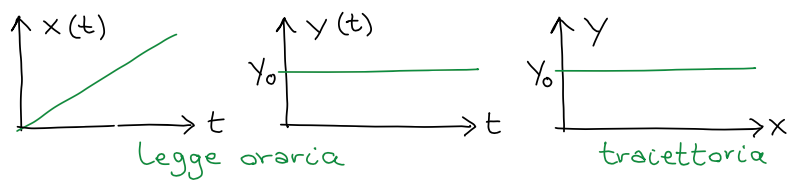
\includegraphics[width=0.8\textwidth]{images/ess-traiettoria.png}
    \end{figure}
\end{example}

\begin{definition}
    La \textbf{velocità istantanea} è la derivata della posizione rispetto al tempo.
    $$v = \lim_{\Delta t \to 0}\frac{\Delta s}{\Delta t} = \frac{ds}{dt}$$
\end{definition}

\begin{definition}
    La \textbf{velocità media} è definita come il rapporto tra lo spostamento e l'intervallo di tempo necessario per effettuarlo.
    $$v_m = \frac{\Delta s}{\Delta t}$$
\end{definition}
\hspace{-15pt}In parole povere è una grandezza che ci dice con quale rapidità cambia la posizione di un punto rispetto al tempo nell'instante $t$.
\subsection*{Vettore velocità}
Derivata rispetto al tempo del vettore posizione e si indica come 
$\frac{d\vec{r}(t)}{dt}\text{ oppure }\dot{\vec{r}}(t)[m/s]$
\begin{equation}
    \begin{split}
    \dot{\vec{r}}(t) & = (\dot{x}(t), \dot{y}(t), \dot{z}(t)) \\
     & = \frac{d}{dt}[x(t)\hat{x} + y(t)\hat{y} + z(t)\hat{z}] \\
     & = \dot{x}(t)\hat{x} + \dot{y}(t)\hat{y} + \dot{z}(t)\hat{z}
    \end{split}
\end{equation}
Per ricavare la forma esplicita uso le proprietà delle derivate (\textbf{linearità}, \textbf{Leibnitz})
\begin{example}
    $\vec{r}(t) = (v_0t, y_0, 0) = v_0t\hat{x} + y_0\hat{y}$ \:\:\:abbiamo che \:\:\:
    $\dot{\vec{r}}(t) = (v_0, 0, 0) = v_0 \hat{x}$
\end{example}
\hspace{-15pt}Velocità e spazio percorso ("integrale di linea").\\
\begin{wrapfigure}[3]{l}{5cm}
    \centering
    \includegraphics[width=5cm]{images/vettore-velocità.png}
\end{wrapfigure}
\begin{align*}
    L & = ||\vec{r}(t_1) - \vec{r}(t_0)|| + ||\vec{r}(t_2) - \vec{r}(t_1)|| + ||\vec{r}(t_3) - \vec{r}(t_2)|| + \dots \\
    & = \sum_i ||\vec{r}(t_{i+1} - \vec{r}(t_i)|| \:\: per\:\: |t_{i+1} - t_i| \text{"piccolo"} \\
    & = \sum_i ||\frac{\vec{r}(t_{i+1}) - \vec{r}(t_i)}{t_{i+1} - t_i}|| (t_{i+1} - t_i) = \int_{t_{in}}^{t_{f_{in}}}||\dot{\vec{r}}(t)||\\
\end{align*}
\begin{example}
    $\vec{r}(t) = (v_0t, y_0)\:\:\: \dot{\vec{r}}(t) = (v_0, 0)$\hspace{15pt}
    $||\dot{\vec{r}}(t)|| = \sqrt{v_0^2 + 0^2} = |v_0|$ \:\:\: $L = |v_0| \cdot (t_{f_{in}} - t_{in})$\\
    Il vettore è costante quindi facendo la derivata torna zero. Con la velocità si calcolo lo spazio percorso ("integrale di linea").
    La differenza fra le posizioni e la differenza dei tempi è il rapporto incrementale in caso gli intervalli siano sufficentemente
    piccoli, da qui si ottiene l'integrale.
\end{example}

\subsection{Vettore accelerazione}
Derivata rispetto al tempo del vettore velocità e si indica con $\frac{d^2\vec{r}(t)}{dt} \text{ oppure } \ddot{\vec{r}}(t) [m/s^2]$
\begin{equation}
    \ddot{\vec{r}}(t) = (\ddot{x}(t), \ddot{y}(t), \ddot{z}(t))\:\: = \:\: \ddot{x}(t)\hat{x} + \ddot{y}(t)\hat{y} + \ddot{z}(t)\hat{z}
\end{equation}
\begin{example}
    $\vec{r}(t)= (\frac{1}{2}a_0t^2, v_0t, 0)$ \hspace{10pt} $\dot{\vec{r}}(t) = (a_0t, v_0, 0)$ \hspace{10pt} $\dot{\vec{r}}(t) = (a_0, 0, 0)$
\end{example}
\hspace{-15pt}Serve perché l'equazione "del moto" di Newton che determinata la legge oraria è formulata in termini di accelerazione.

\subsection{Vettore quantità di moto}
Il prodotto di massa [kg] e velocità [m/s]
$$\vec{p}(t) = m \cdot \dot{\vec{r}}(t) = (m\dot{x}(t), m\dot{y}(t), m\dot{x}(t)) = m\dot{\vec{x}}(t)x + m\dot{\vec{y}}(t)y + m \dot{\vec{z}}(t)z$$
\begin{example}
    Prendiamo un punto di massa 2kg e velocità 3m/s lungo $\hat{x}$.\\
    $p_x(t) = 2 \cdot 3 kg\cdot m/s = 6 kg \cdot m/s$ \hspace{15pt} $p_y(t) = p_z(t) = 0$.
\end{example}
\hspace{-15pt}Serve per generalizzare l'equazione di Newton e per trattare sistemi di piu punti materiali.

\subsection{Vettore momento angolare rispetto a un polo P}
$$\vec{L}_p(t) = m(\vec{r}(t) - \vec{r}_p) \times \dot{\vec{r}}(t)$$
Dove $\vec{r}_p$ è il vettore posizione di p, mentre $\dot{\vec{r}}(t)$ è il prodotto vettoriale.
\begin{example}
    $\vec{r}_p = (l_0, 0, 0)$ \hspace{15pt} $\vec{r}(t) = (v_0t, y_0, 0)$\\
    $\vec{L}_p = m[(v_0t - l_0)\hat{x} + y_0\hat{y}] \times (v_0\hat{x}) \:\: = \:\: m(v_0t - l_0)v_0 \hat{x} \times \hat{x} + my_0v_0\hat{y}\times \hat{x} 
    \:\: = \:\: my_0v_0(-\hat{z}) = (0,0, -my_0v_0)$\\
    Ricorda che $\hat{x} \times \hat{x} = 0$ e $\hat{y} \times \hat{x} = -\hat{z}$
\end{example}
\hspace{-15pt}Il momento angolare dice quanta inerzia ha un oggetto in una rotazione (descrizione sommaria).\\
Il polo P è parte della definizione. È una scelta! Il risultato dipende dal polo.
Serve per formulare l'equazione del moto di sistemi di punti materiali e corpi rigidi.

\subsection{Coordinate polari}
Un metodo per rapprensentare delle cordinate x, y andando a misurare prima la distanza dall'origine e poi si va a vedere
quanto vale l'angolo fra questo segmento dall'asse x, utilizzando seno e coseno.
\begin{wrapfigure}[7]{l}{2cm}
    \centering
    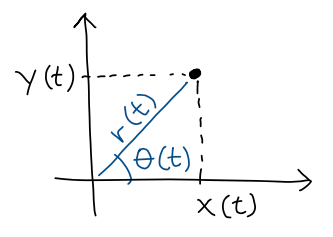
\includegraphics[width=5.5cm]{images/coordinate-polari.png}
\end{wrapfigure}
\begin{align*}
    \begin{cases}
        x(t) = r(t) \cdot \cos(\Theta(t))\\
        y(t) = r(t) \cdot \sin(\Theta(t)) 
    \end{cases}
\end{align*}
\begin{align*}
    \begin{cases}
        r(t) = \sqrt{x(t)^2 + y(t)^2} \geq 0\\
        tg(\Theta(t)) = y(t) / x(t) 
    \end{cases}
\end{align*}
\\
\begin{example} Esempi di rappresentazione di coordinate in coordinate polari.\\
    $x = 0, y = l_0 > 0 \:\: \Rightarrow \:\: r = l_0, \Theta = \pi/2$\\
    $x = 0, y = -l_0 < 0 \:\: \Rightarrow \:\: r = l_0, \Theta = -\pi/2$\\
    $x = l_0, y = l_0 > 0 \:\: \Rightarrow \:\: r = \sqrt{2}l_0, \Theta = \pi/4$\\
\end{example}

\subsection{Versori polari (2D)}
Definisco un versore $\hat{r}(t)$ che punta verso il punto materiale e un versore $\hat{\Theta}(t)$ ortogonale.
Si esprime facilmente in coordinte polari.
$$\vec{r}(t) = (x(t), y(t)) = (r(t)\cos \Theta(t), r(t)\sin\Theta(t)) \:\: = \:\: r(t)(\cos\Theta(t)\hat{x} + \sin\Theta(t)\hat{y})$$
Ma $||\vec{r}(t)|| = |r(t)| = r(t)$ allora definisco $\hat{r}(t) = \vec{r}(t)/ ||\vec{r}(t)|| = \cos \Theta(t)\hat{x} + \sin\Theta(t)\hat{y}$\\\\
Trovo facilmente che un versore ortogonale è:
$$\hat{\Theta(t)} = -\sin\Theta(t)\hat{x} + \cos\Theta(t)\hat{y} \:\:\:\text{infatti} \:\:\: \hat{r}\cdot \hat{\Theta} = c \cdot (-s) + s \cdot c = 0$$
\begin{wrapfigure}[7]{r}{6cm}
    \centering
    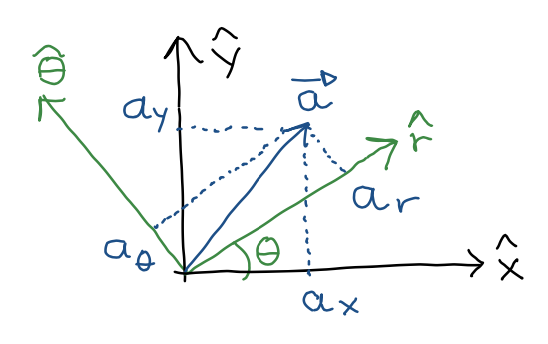
\includegraphics[width=5.5cm]{images/trasformazioni-inverse.png}
\end{wrapfigure}
\begin{note}
    Non c'è legame fra $\Theta$ e $\hat{\Theta}$ è solo una convenzione.
\end{note}
\hspace{-15pt}Le trasformazioni inverse invece si fanno come segue (verifico per sostituzione):
$$\hat{y} = \cos\Theta(t)\hat{r} - \sin\Theta(t)\hat{\Theta} \hspace{20pt} \hat{y} = \sin\Theta(t)\hat{r} + \cos\Theta(t)\hat{\Theta}$$
Possono quindi scrivere ogni vettore nella forma $\vec{a} = a_r\hat{r} + a_{\Theta}\hat{\Theta}$ con le componenti polari $a_r, a_{\Theta}$.
Per evitare ambiguità non scriviamo $(a_r, a_{\Theta})$ e riserviamo la notazione alle componenti cartesiane.\\\\
A differenza dei versori cartesiani quelli polari dipendono dal tempo per costruzioni.
$$\dot{\hat{r}}(t) = \frac{d}{dt}[\cos\Theta(t) \hat{x} + \sin\Theta(t)\hat{y}] \:\: = \:\: -\sin\Theta(t) \cdot \dot{\Theta}(t)\hat{x} + \cos\Theta(t) \cdot \dot{\Theta}(t)\hat{y}$$
Dove $\cos\Theta(t) \cdot \dot{\Theta}(t)$ si applica la derivata della somma, Leibnitz, funzione composta.
$$= \dot{\Theta}(t)\cdot \hat{\Theta}(t) \:\:\:\:(\text{confronto l'espressione di} \hat{\Theta}(t))$$
Similmente $\dot{\hat{\Theta}}(t)= - \dot{\Theta}\hat{r}(t)$.


\subsection*{Vettori posizione, velocità, accelerazione}
$$\vec{r}(t) = r(t)\hat{r}(t)$$
Dove abbiamo che $\vec{r}(t)$ è il vettore, $r(t)$ è una coordinata polare, $\hat{t}(t)$ è il versore polare.
$$\dot{\vec{r}}(r) = \dot{r}(t)\hat{r}(t) + r(t)\dot{\Theta}(t)\hat{\Theta}(t)$$
Dove la parte $\dot{\vec{r}}(r)$ è la velocità radiale.
$$\ddot{\vec{r}}(t) = [\ddot{r}(t) - r(t)\dot{\Theta}(t)^2] \hat{r} + [r(t) \ddot{\Theta}(t) + 2\dot{r}(t)\dot{\Theta}(t)]\hat{\Theta}$$
Nel quale abbiamo che la parte $r(t)\dot{\Theta}(t)^2$ si chiama \textbf{velocità centripeta}, mentre $2\dot{r}(t)\dot{\Theta}(t)$ si dice \textbf{accelerazione di Coriolis}.


	% !TeX spellcheck = it_IT
\newpage
\section{Processo software}
\begin{definition}[Processo software]
	Sequenza di attività necessarie a sviluppare un sistema software.
\end{definition}
\noindent Ogni modello di processo software include:
\begin{itemize}
	\item \textbf{Specifica}: definizione di cosa deve essere fatto
	\item \textbf{Progettazione} e \textbf{implementazione}
	\item \textbf{Validazione}: verifica che il sistema rispetti le specifiche
	\item \textbf{Evoluzione}: modifica o aggiornamento del sistema
\end{itemize}

\subsection{Fasi di sviluppo}
\subsubsection{Specifica}
Questa fase stabilisce quali \textbf{servizi} sono richiesti e quali \textbf{vincoli} ci sono. È quindi un processo di \textit{ingegneria dei requisiti}:
\begin{itemize}
	\item \textbf{Estrazione} e \textbf{analisi} dei requisiti: cosa richiedono o si aspettano gli stakeholder
	\item \textbf{Specifica} dei requisiti: definirli in dettaglio
	\item \textbf{Convalida} dei requisiti: verificare che siano validi
\end{itemize}
\begin{center}
	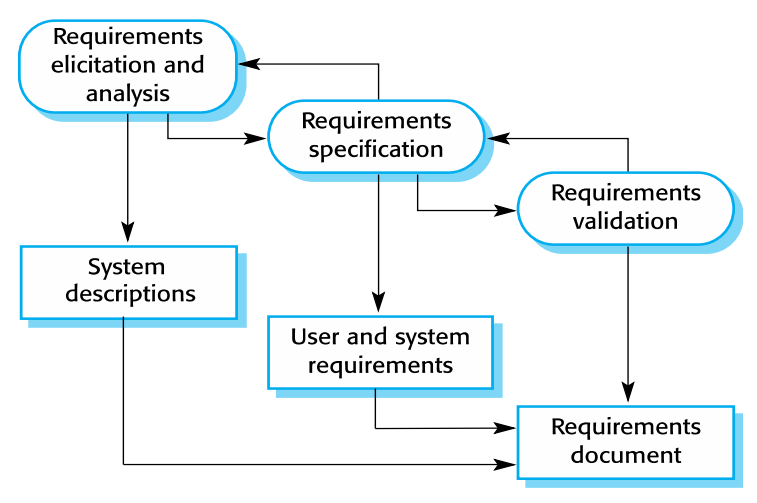
\includegraphics[scale=0.4]{specifica.png}
\end{center}

\subsubsection{Progettazione}
In questa fase si definisce una struttura software che realizzi la specifica, analizzando quattro aspetti:
\begin{itemize}
	\item \textbf{Architectural design}: identificazione della struttura in termini di componenti e di come si relazionano tra di loro
	\item \textbf{Database design}: definizione delle strutture dati necessarie e della loro rappresentazione in database
	\item \textbf{Interface design}: definizione delle interfacce tra le diverse componenti del sistema
	\item \textbf{Component design}: definizione in dettaglio delle varie componenti, identificando quelle realizzabili con elementi già esistenti
\end{itemize}
\begin{center}
	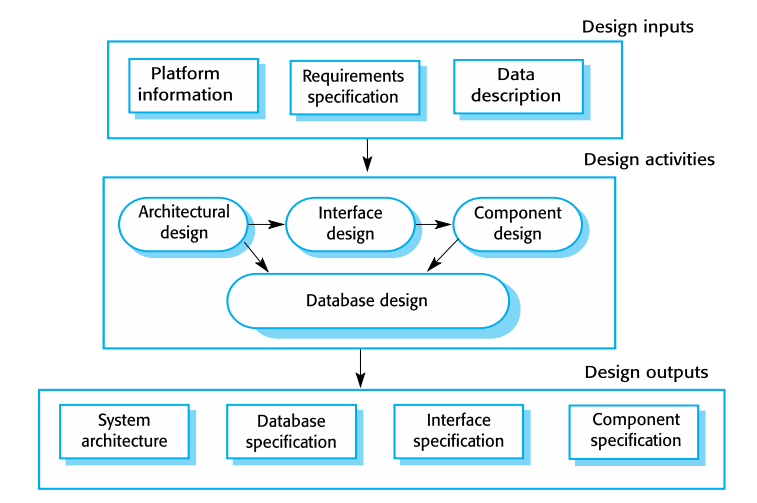
\includegraphics[scale=0.4]{prog.png}
\end{center}

\subsubsection{Sviluppo}
La struttura progettata nella fase precedente viene ora realizzata tramite uno o più applicativi da implementare o da configurare. Include:
\begin{itemize}
	\item \textbf{Programmazione} attività senza un processo standard
	\item \textbf{Debugging}: attività per identificare e correggere errori o bug
\end{itemize}
Spesso la progettazione e lo sviluppo sono svolte in \textbf{interleaving}.

\subsubsection{Validazione}
\textbf{Verifica} e \textbf{validazione} hanno lo scopo di dimostrare che un sistema è conforme alle specifiche e soddisfa i requisiti del cliente. Viene spesso fatta tramite \textbf{testing} con casi derivati dalla specifica dei dati che poi dovranno essere realmente utilizzati. Si suddivide in:
\begin{itemize}
	\item \textbf{Component} testing: i componenti sviluppati sono testati indipendentemente
	\item \textbf{System} testing: il sistema è testato interamente prestando particolare attenzione alle \textit{emergent properties}
	\item \textbf{Customer} testing: il sistema è testato con i dati del cliente
\end{itemize}
\begin{center}
	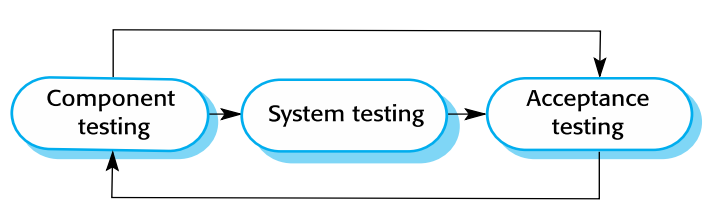
\includegraphics[scale=0.4]{valida.png}
\end{center}

\subsubsection{Evoluzione}
I cambiamenti sono inevitabili in quanto le richieste del cliente possono cambiare nel tempo o possono uscire nuove tecnologie più aggiornate. Questi portano a dei \textbf{rework} costosi che richiedono la ripetizione parziale delle fasi precedentemente descritte.\\
Per ridurre i costi è importante anticipare i cambiamenti e garantire quindi \textbf{change tolerance}. Questo è più facile con i modelli incrementali.

\subsection{Modelli}
\begin{definition}[Modello]
	Il modello di un processo software fornisce una rappresentazione astratta del processo stesso:
	\begin{itemize}
		\item \textbf{Suddivisione} del processo in attività: cosa fare, quando farlo, come e cosa si ottiene
		\item \textbf{Organizzazione} delle attività: ordinamento, criteri di terminazione
	\end{itemize}
	E.g. ISO 12207
\end{definition}

\subsubsection{Sequenziale}
\paragraph{Build and fix}
Questo modello non prevede alcuna specifica o progettazione: lo sviluppatore scrive un programma e lo modifica ripetutamente finché non soddisfa il cliente. Adeguato solo per progetti molto piccoli.
\begin{center}
	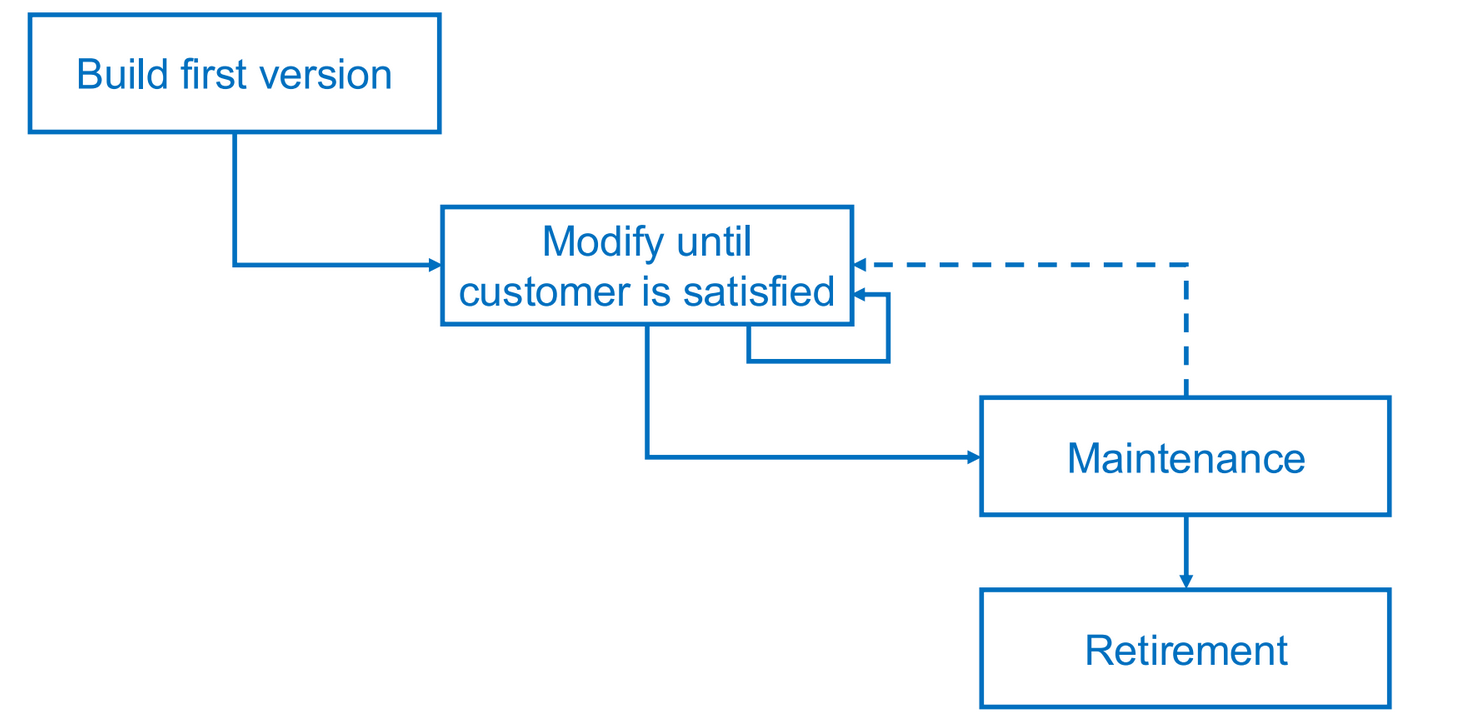
\includegraphics[scale=0.15]{buildfix.png}
\end{center}

\paragraph{Modello a cascata}
Modello ideato da Royce nel 1970, fu il primo a distinguere e definire le fasi di un processo software, dando finalmente importanza all'analisi e alla progettazione prima della codifica.\\
Ogni fase prima di procedere deve produrre un documento che deve essere approvato da chi di dovere.\\
I \textbf{contro} principali sono l'enorme quantità di \textit{documenti} prodotti e l'estrema \textit{rigidità}: il cliente vede solo il prodotto finale che spesso non va bene e si deve rincominciare da capo.

\begin{center}
	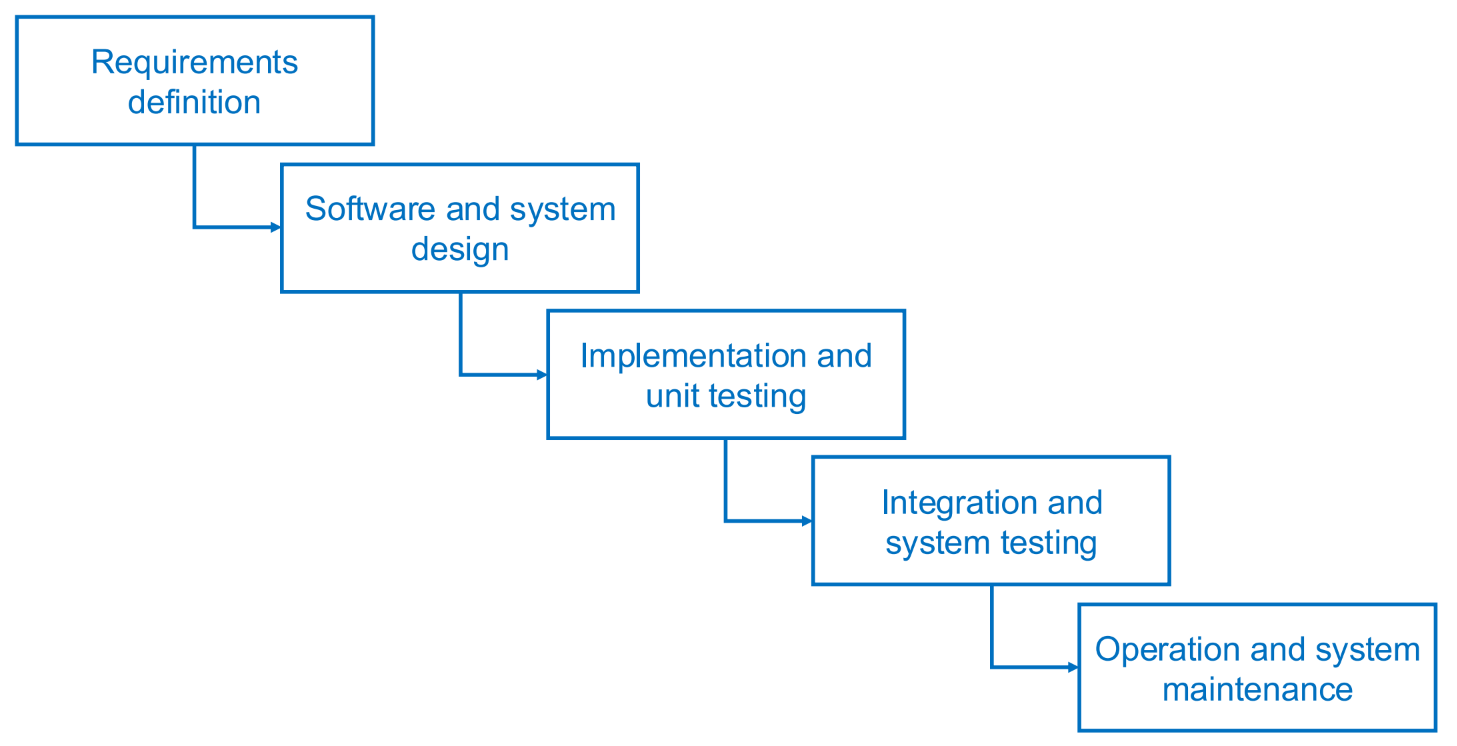
\includegraphics[scale=0.15]{royce.png}
\end{center}

\begin{note}
	Royce stesso riconosce i problemi del suo modello e propone un alternativa con un \textbf{feedback loop} da una fase alla precedente.
\end{note}

\paragraph{Modello a V}
In questo modello le attività di \textbf{sinistra} sono di analisi che scompongono i requisiti degli utenti in sezioni piccole; quelle di \textbf{destra} aggregano e testano il prodotto delle precedenti per verificare che le esigenze siano effettivamente rispettate.\\
Al centro troviamo la progettazione dei \textbf{test} da eseguire prima della codifica.
\begin{center}
	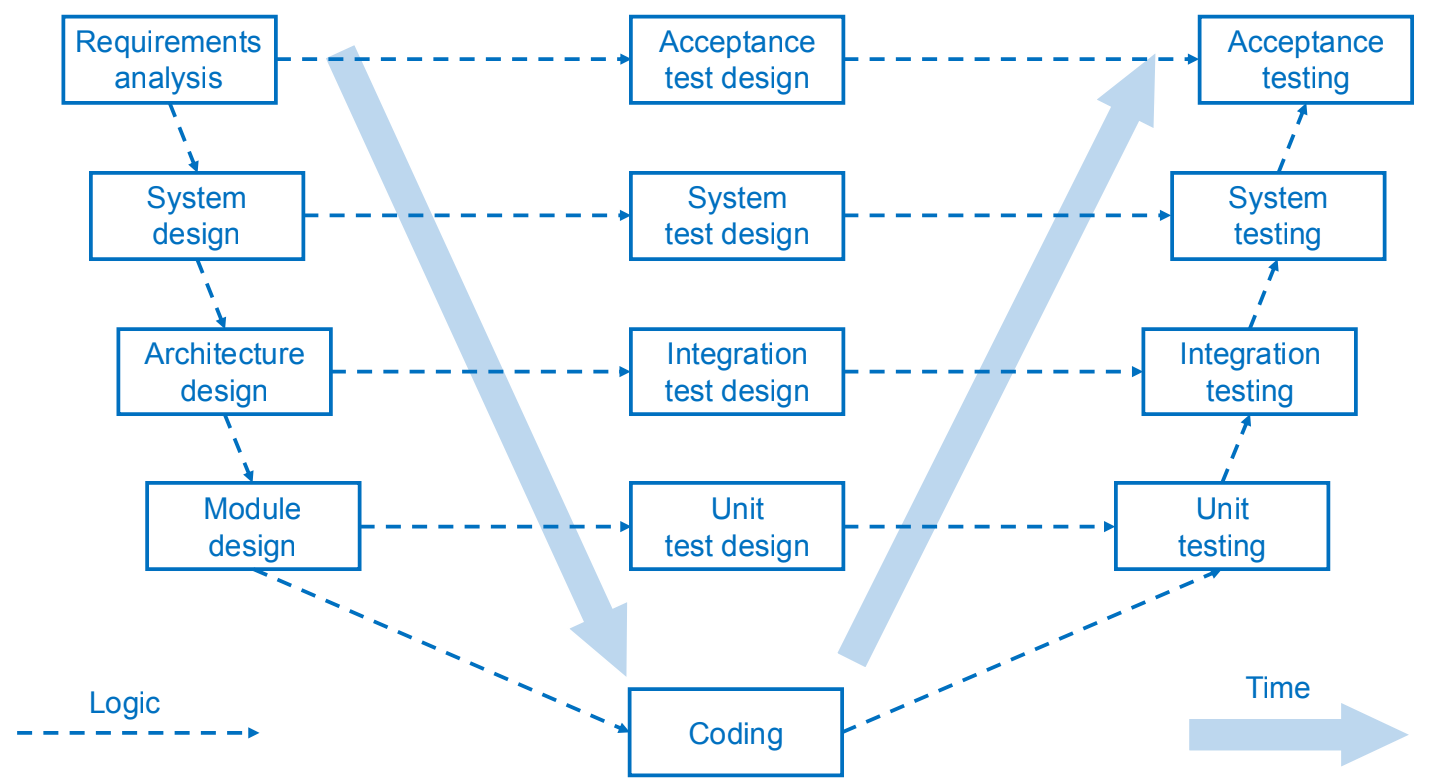
\includegraphics[scale=0.3]{Vmodel.png}
\end{center}

\begin{note}
	Questo modello è uno standard SQA (qualità del software).
\end{note}

\subsubsection{Iterativo}
\paragraph{Rapid prototyping o evolutivo}
Consiste nel costruire velocemente un prototipo per permettere al committente di sperimentarlo. In questo modo il cliente può descrivere meglio i requisiti, sopratutto quando anche a lui non sono chiari.
\begin{center}
	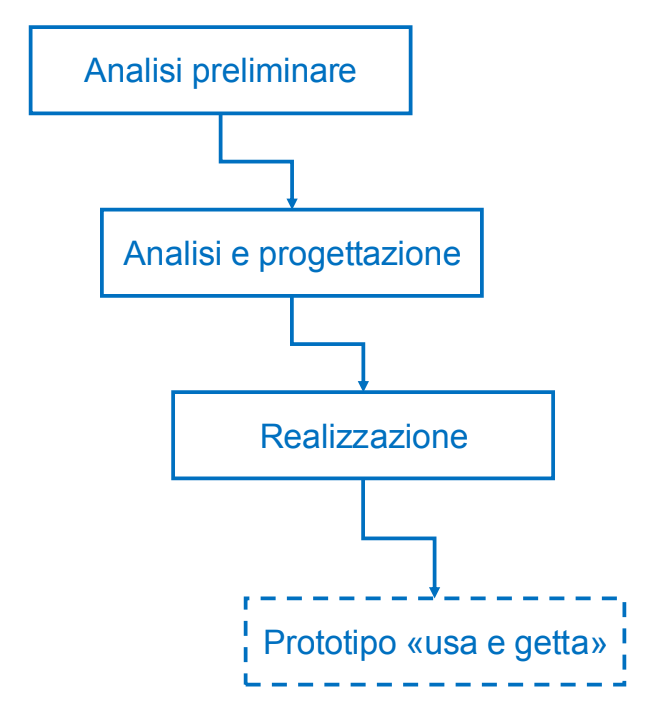
\includegraphics[scale=0.3]{rapidproto.png}
\end{center}

\paragraph{Modello incrementale}
In questo modello il sistema è costruito \textbf{iterativamente} aggiungendo nuove funzionalità a partire da requisiti definiti inizialmente.\\
Questo permette di \textbf{ritardare} fasi che per motivi esterni non possono proseguire e fa uscire versioni iniziali ed utilizzabili molto rapidamente, in modo da ricevere anche \textbf{feedback} che aiutino a correggere il prodotto a basso costo.\\
I contro principali sono che il processo di sviluppo non è molto visibile e c'è il rischio che diventi un \textit{build and fix}: la struttura del sistema tende a degradarsi e diventa più costoso fare il refactoring.

\begin{center}
	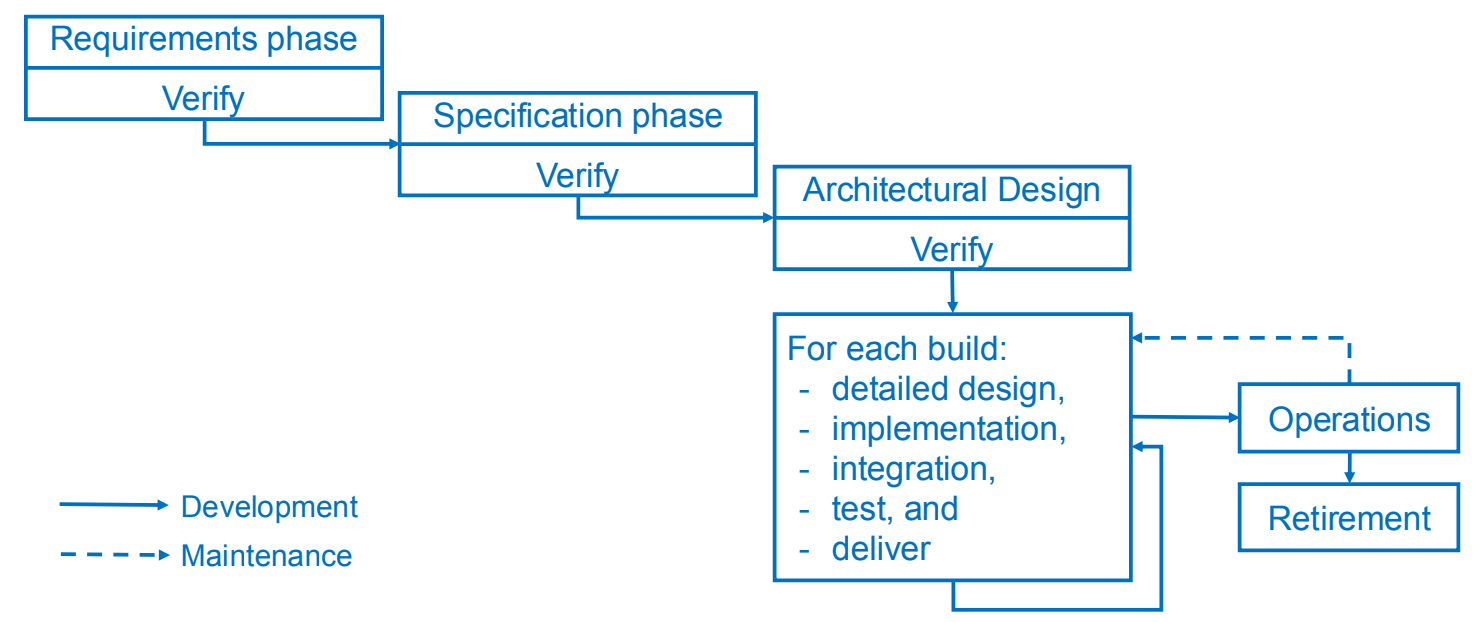
\includegraphics[scale=0.3]{incrementale.png}
\end{center}

\paragraph{Modello a spirale}
Ideato da Bohem nel 1998, ispirato dal \textit{plan-do-check-ackt} di Deming, divide ogni \textbf{iterazione} in quattro fasi:
\begin{enumerate}
	\item Definizione degli obiettivi
	\item Analisi dei rischi
	\item Sviluppo e validazione
	\item Pianificazione del nuovo ciclo
\end{enumerate}
È un modello astratto da istanziare decidendo cosa fare in ogni iterazione e in ogni fase, applicandolo volendo ai cicli tradizionali. Si concentra molto sugli aspetti gestionali: pianificazione delle fasi, \textbf{risk-driven} (guidato dall'analisi dei rischi) e comunicazione con il cliente.

\begin{center}
	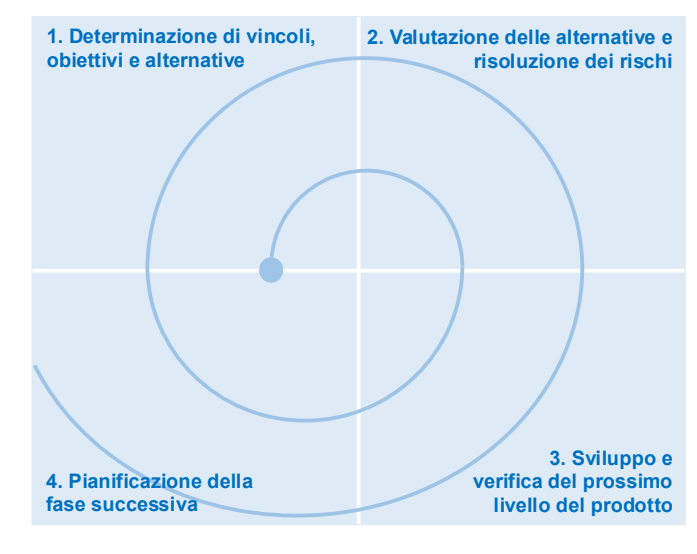
\includegraphics[scale=0.4]{spirale.png}
\end{center}

\paragraph{Unified process}
Ideato da Booch Et Al nel 1999, è guidato da \textbf{casi d'uso} e \textbf{analisi dei rischi} già a partire dalla raccolta e analisi dei requisiti. È un modello iterativo \textbf{incrementale} incentrato sull'\textbf{architettura}: nelle prime fasi c'è una definizione generale e i dettagli vengono lasciati alle fasi successive. Questo permette di avere subito una visione generale del sistema che diventa poi facilmente adattabile.
\begin{center}
	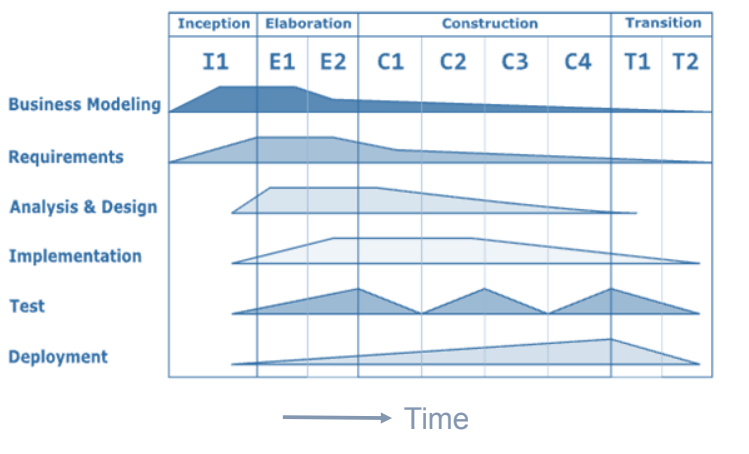
\includegraphics[scale=0.5]{unifproc.png}
\end{center}

\subsubsection{Agile}
Oggi è sempre più importante la \textbf{rapidità} nello sviluppo e nel rilascio del software in quanto i requisiti delle aziende cambiano molto velocemente e con essi diventa impossibile avere un sistema stabile di requisiti.\\
Il modello agile viene introdotto negli anni '90 proprio per ridurre i tempi sopra descritti:
\begin{itemize}
	\item Le fasi di specifica, progettazione e sviluppo sono eseguite in \textbf{interleaving}
	\item Il sistema è sviluppato con versioni incrementali valutate assieme agli stakeholder
	\item Rilascio frequente
	\item Supporti allo sviluppo, e.g. automated testing
\end{itemize}
\begin{center}
	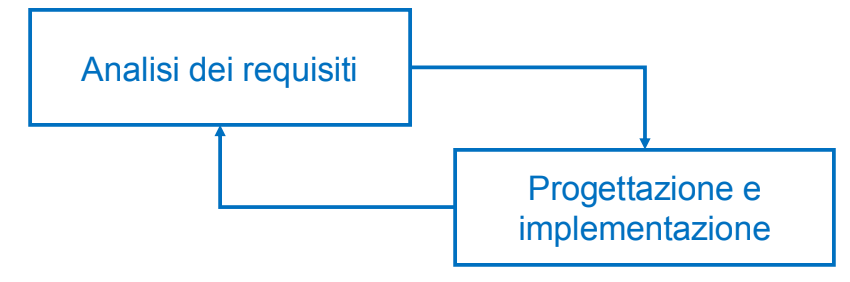
\includegraphics[scale=0.3]{agile.png}
\end{center}

Il modello agile segue i seguenti principi:
\paragraph{Customer involvement} I clienti devono essere coinvolti durante il processo di sviluppo per fornire, prioritizzare e valutare le iterazioni del sistema.
\paragraph{People not process} Le abilità del team devono essere riconosciute e gli sviluppatori devono essere liberi di sviluppare a modo loro, purché venga mantenuta comunicazione.
\paragraph{Mantain semplicity} Cercare di ridurre sempre al minimo la complessità nello sviluppo e nel sistema. Bisogna mantenere il codice semplice ma avanzato tecnicamente a discapito di una documentazione mantenuta al minimo.
\paragraph{Incremental delivery} Il sistema software è sviluppato in versioni incrementali, con il cliente che specifica i requisiti da soddisfare in ciascuna versione.
\paragraph{Embrace change} Accettare che i requisiti cambieranno nel tempo e rendere facile la loro implementazione.\\\\

Il modello agile è \textbf{conveniente} per lo sviluppo di prodotti di piccola o media dimensione (fino a $50$ sviluppatori) oppure in contesti di sviluppo di sistemi custom (meno regolamenti e restrizioni).\\
Nella pratica comunque viene usato nella maggior parte dei team.\\\\

\noindent Il modello agile ha portato alla nascita di:
\begin{itemize}
	\item \textbf{Continuous Integration}: integrazione continua di tutte le modifiche o aggiunte all'interno di un \textit{main branch}, validata tramite automatic build e testing
	\item \textbf{Continuous deployment}: dispiegamento continuo e \textit{automatico} delle nuove versioni ottenute tramite CI
\end{itemize}

\subsubsection{Extreme Programming}
L'extreme programming è un approccio estremo all'approccio iterativo e agile. Prevede che nuove versioni minori siano rilasciate più volte in un giorno, versioni incrementali rilasciate al cliente ogni due settimane e tutti i test sono eseguiti per ogni build.
\begin{center}
	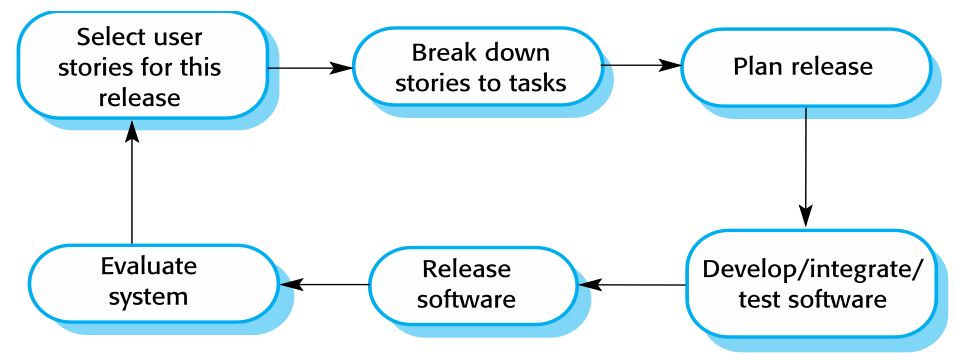
\includegraphics[scale=0.35]{xp.png}
\end{center}

\noindent Alcune pratiche comuni nell'XP:
\paragraph{Planning incrementale} I requisiti sono raccolti sotto forma di user stories divise in \textbf{task}. Quelle da includere nella release sono determinate in base al tempo disponibile e alla loro priorità.
\paragraph{Release piccole} Si parte con una piccola release iniziale che garantisca le funzionalità di base si procede con piccole e frequenti release che aggiungono funzionalità.
\paragraph{Design semplice} La progettazione si concentra solo sui requisiti correnti e deve essere comprensibile a tutti.
\paragraph{Test-first developement} Si sviluppano prima i test del codice stesso (a volte generati automaticamente).
\paragraph{Refactoring} Il refactoring deve essere eseguito continuamente appena ci si rende conto del miglioramento necessario, mantenendo sempre il codice semplice, facilmente manutenibile e auto esplicativo.
\paragraph{Pair programming} Gli sviluppatori lavorano in coppia in modo che ci sia sviluppo e supporto reciproco.
\paragraph{Collective ownership} Le coppie lavorano su tutte le aree del sistema e la responsabilità è quindi condivisa.
\paragraph{Sustainable pace} Ridurre al minimo il lavoro straordinario in quanto abbassa qualità e produttività.
\paragraph{On-site customer} Un rappresentante del cliente deve essere disponibile al team per fornire o prioritizzare i requisiti.\\\\

Il modello di Extreme Programming si concentra principalmente su aspetti tecnici e per questo non è facilmente integrabile nelle organizzazioni. Di conseguenza il metodo non è molto diffuso ma alcuni degli aspetti che tratta sono stati trasportati in altri approcci.

\subsubsection{Scrum}
Scrum è un metodo agile per lo sviluppo iterativo e incrementale di un sistema software. L'idea è di ottenere un processo in cui un insieme di persone si muovono all'unisono per raggiungere un obiettivo che soddisfi la squadra.
\begin{definition}[Product backlog]
	Documento che contiene tutti i requisiti attualmente conosciuti.
\end{definition}
Ci sono tre figure coinvolte:
\begin{itemize}
	\item \textbf{Product owner}: chi identifica le caratteristiche del prodotto, decide le priorità e revisiona il \textbf{product backlog} per assicurarsi che vengano rispettati i requisiti
	\item \textbf{Scrum master}: figura responsabile di assicurare che il processo avvenga efficacemente, garantendo le condizioni ambientali e motivazionali al meglio assicurandosi che non ci siano interferenze esterne (senza però avere autorità sul team)
	\item \textbf{Developement team}: gruppo autogestito di sviluppatori non più grande di 7 persone che si occupa dello sviluppo e della documentazione
\end{itemize}
Le fasi del metodo scrum sono:
\begin{enumerate}
	\item \textbf{Pre-game phase}, ovvero la pianificazione, che a sua volta si compone di:
	\begin{itemize}
		\item \textbf{Planning sub-phase}: definizione del sistema che deve essere sviluppato in termini di product backlog
		\item \textbf{Architecture sub-phase}: design di alto livello del sistema, inclusa l'architettura, in base agli elementi del backlog
	\end{itemize}
	\item \textbf{Game phase}, ovvero lo sviluppo. Il sistema viene sviluppato attraverso una serie di \textbf{sprint}, ovvero un ciclo iterativo nel quale vengono sviluppate o migliorate delle funzionalità. Ogni sprint dura da una settimana ad un mese e include le classiche fasi di sviluppo. Si divide nelle seguenti fasi:
	\begin{enumerate}
		\item Si parte dal product backlog che contiene la lista dei \textbf{requisiti} da fare (TBD). Da questi vengono selezionati dal team e dal cliente quelli da sviluppare.
		\item Si procede con la pianificazione, gestita dal product owner, e con la creazione dello \textbf{sprint backlog}
		\item Inizia lo sviluppo da parte dei diversi team che rimangono isolati e protetti dallo scrum master; si occupa anche di organizzare brevi meeting giornalieri di aggiornamento.
		\item Al termine dello sprint il prodotto viene revisionato in un incontro tra team, clienti ed eventuali utenti
		\item Tra uno sprint ed il successivo viene organizzato un evento di \textbf{retrospettiva} dove il team riflette, impara e si adatta con l'obiettivo di migliorare
	\end{enumerate}
	\item \textbf{Post-game phase}: conclude il processo di sviluppo e il prodotto viene preparato per il rilascio (test, integrazione, documentazione, formazione e marketing)
\end{enumerate}
I vantaggi di questo approccio sono che il prodotto e \textbf{partizionato} in sotto problemi più facili da gestire, i requisiti non ancora pronti non ostacolano lo sviluppo, c'è molta comunicazione, i clienti ottengono increment periodici e si stabilisce un rapporto di fiducia.

\subsection{Kanban}
Il Kanban è un approccio all'organizzazione di un progetto che consiste nel dividere le attività tra \textbf{To Do}, \textbf{Work In Progress} e \textbf{Done}. Questi vengono poi visualizzati tramite una tabella. Viene inoltre imposto un limite alla categoria WIP che riduce il \textbf{task switching} e rende più facile trovare i colli di bottiglia. Ottimizza in generale l'\textbf{efficienza}.
	% !TeX spellcheck = it_IT
\newpage
\section{Analisi dei requisiti}
\begin{definition}
	Processo di studio e analisi delle esigenze del committente e dell'utente per giungere alla definizione del dominio del problema e dei requisiti del sistema.
\end{definition}
L'analisi serve a capire \textbf{cosa} fare e non come farlo, identificando i confini del sistema SW, il modo in cui interagisce con l'ambiente e la qualità con cui lo fa.\\
È un processo \textbf{fondamentale} in quanto permette di individuare e risolvere difetti in maniera meno costosa rispetto alle altre fasi di sviluppo software.\\
Il prodotto dell'analisi dovrà essere un documento e/o modello che descrive il \textbf{dominio} del sistema, i suoi \textbf{requisiti} ed opzionalmente il \textit{manuale utente} e i \textit{casi di test}.
\subsection{Studio di fattibilità}
È la fase preliminare per stabilire l'opportunità di realizzare o meno un sistema software. Si basa su:
\begin{itemize}
	\item \textbf{Descrizione} del sistema e delle necessità degli utenti
	\item Analisi di \textbf{mercato}:
	\begin{itemize}
		\item Mercato \textit{attuale} e \textit{futuro}
		\item \textit{Costo} di produzione
		\item \textit{Redditività} attesa
	\end{itemize}
	\item Analisi tecnica di \textbf{realizzabilità}:
	\begin{itemize}
		\item Strumenti necessari
		\item Soluzioni algoritmiche e architetturali
		\item Hardware
		\item Processo
	\end{itemize}
\end{itemize}

\subsection{Dominio}
Per la costruzione del dominio sono necessari:
\begin{itemize}
	\item Un \textbf{glossario}: collezione di termini rilevanti al caso specifico. Costruito strada facendo dagli analisti e può essere riutilizzato.
	\item Modello \textbf{statico} e \textbf{dinamico}
\end{itemize}
Ci si deve concentrare su: \textbf{entità}, \textbf{relazioni}, \textbf{processi} e \textbf{comportamenti}.

\begin{example}[House of cars]
	House of Cars è un parcheggio verticale multipiano, formato da 10 colonne e 24 piani per colonna, 12 sotto al livello strada e 12 sopra.
	
	\paragraph{Glossario}
	\begin{itemize}
		\item \textit{Colonna}: colonna di posti auto dotata di un sollevatore centrale che raggiunge tutti i piani del parcheggio; ha un proprio locale di ricezione auto; comprende un carrello
		\item \textit{Carrello}: carrello per movimentare le vetture; è dotato di “forchette” in corrispondenza delle ruote
		\item \textit{Cella}: formata da due box affiancati: può quindi contenere due auto
		\item \textit{Gruppo di spostamento elettromeccanico}: controlla il carrello che trasla la vettura nelle celle posizionate davanti e dietro al sollevatore
		\item  $\ldots$
	\end{itemize}
	
	\begin{center}
		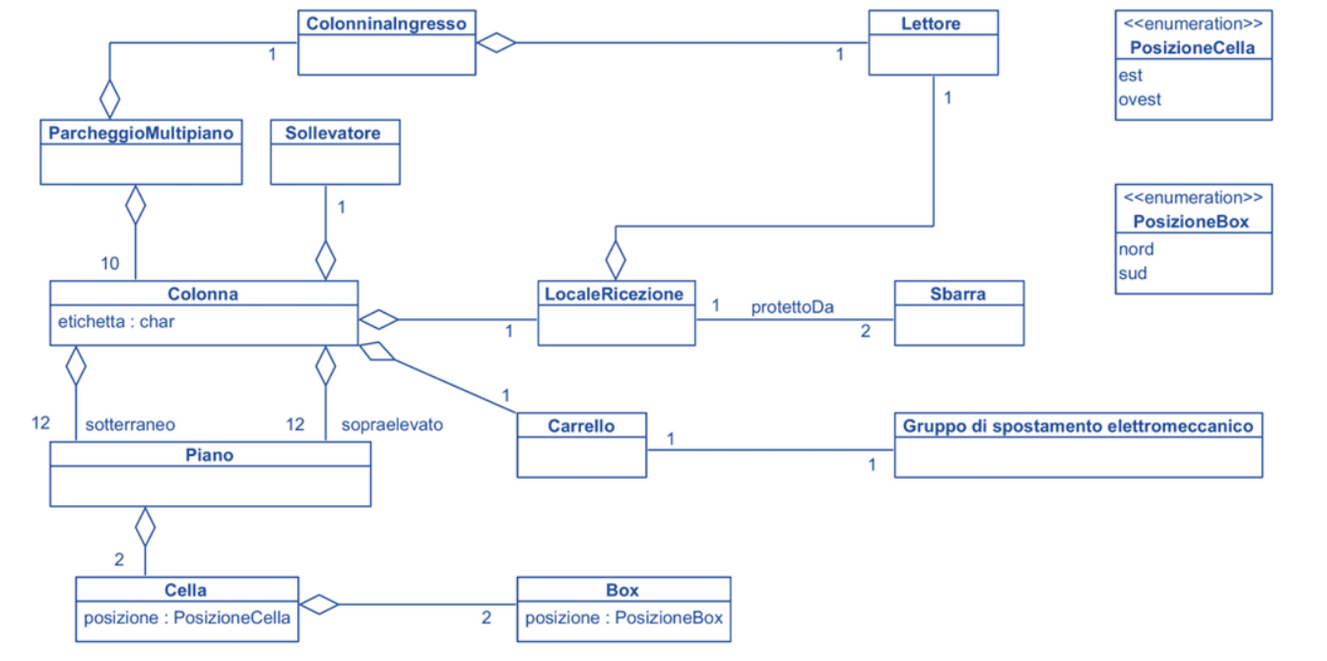
\includegraphics[scale=0.3]{smodelhousecars.png}
		\captionof{figure}{Modello statico}
	\end{center}
	\begin{center}
		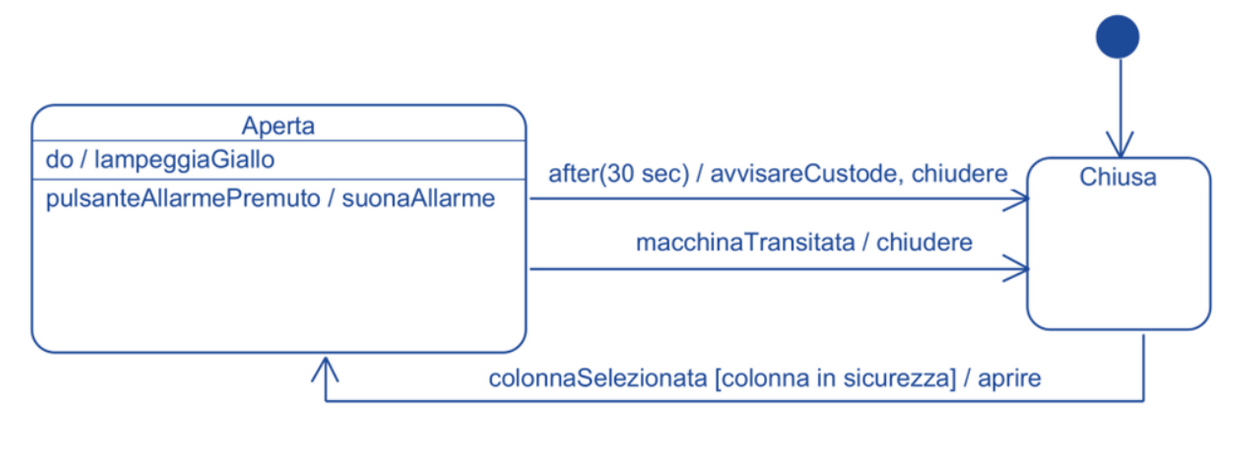
\includegraphics[scale=0.3]{dmodellohousecars.png}
		\captionof{figure}{Modello dinamico}
	\end{center}
\end{example}

\subsection{Requisiti}
Un requisito è una proprietà che deve essere garantita dal sistema per soddisfare una necessità dell'utente.
\begin{definition}[IEEE definition]
	Un requisito è:
	\begin{itemize}
		\item Una condizione (o capacità) necessaria a un utente per risolvere un problema o raggiungere un obiettivo
		\item Una condizione (capacità) che deve essere soddisfatta/posseduta da un sistema per soddisfare un contratto, uno standard, una specifica, o altri documenti formali
	\end{itemize}
\end{definition}
\noindent I requisiti possono essere di due tipi (che devono rimanere separati):
\begin{itemize}
	\item \textbf{Funzionali}: descrivono le \textbf{funzionalità} che il sistema deve realizzare in termini di \textit{azioni}, \textit{risposte agli input} e \textit{comportamenti in casi particolari}.
	\item \textbf{Non funzionali}: descrivono le \textbf{proprietà} del SW:
	\begin{itemize}
		\item \textbf{qualità}, e.g. efficienza, affidabilità, sicurezza
		\item \textbf{processo}, e.g. standard di processo, linguaggi usati, metodo di sviluppo
		\item \textbf{esterne}, e.g. interoperabilità e vincoli legislativi
		\item \textbf{fisici}, e.g. hardware, rete
	\end{itemize}
\end{itemize}
\begin{observation}
	Un requisito deve essere \textbf{ben posto}, idealmente nella forma \textbf{assertiva}
	\begin{equation*}
		\text{Il } <\text{sistema}>\text{ deve }<\text{funzionalità/proprietà}>
	\end{equation*}
\end{observation}

\begin{definition}[Documento dei requisiti]
	È un documento che specifica \textbf{cosa} deve fare il sistema e con quali \textbf{vincoli}. È un contratto tra lo sviluppatore e l'utente che in genere specifica anche la scadenza.
\end{definition}

\subsubsection{Acquisizione}
L'acquisizione può avvenire in diversi modi:
\begin{itemize}
	\item \textbf{Interviste}
	\begin{itemize}
		\item \textit{Strutturate}
		\item \textit{Non strutturate}
	\end{itemize}
	\item \textbf{Questionari} a risposta multipla
	\item Costruzione di \textbf{prototipi} (anche su carta)
	\item \textbf{Osservazione} di futuri utenti al lavoro: i \textbf{casi d'uso} devono includere la sequenza di eventi corretta ed eventuali comportamenti inattesi
	\item \textbf{User stories}: utilizzato nei processi \textit{Agile}, i requisiti sono descritti con un template predefinito
	\begin{equation*}
		\text{As a} <\text{user role}>\text{ I want }<\text{goal}>\text{ so that }<\text{benefit}>
	\end{equation*}
	che viene messo su un foglio in formato $A6$ (facile, visibile e rende possibile appenderli e collegarli). Questa tecnica però non è \textbf{scalabile}, è \textbf{vaga} e \textbf{informale} e spesso non include dettagli sui requisiti \textbf{non funzionali}.
	\item \textbf{Studio} di documenti
\end{itemize}

\subsubsection{Elaborazione}
Durante questa fase i requisiti vengono \textbf{espansi} e \textbf{raffinati} e viene scritta la prima bozza del documento. Questo deve essere strutturato in:
\begin{enumerate}
	\item \textbf{Introduzione}: perché il sistema è desiderabile e come si inquadra negli obiettivi più generali del cliente
	\item \textbf{Glossario}
	\item \textbf{Requisiti funzionali}
	\item \textbf{Requisiti non funzionali}
	\item \textbf{Architettura}: strutturazione in sottoinsiemi
	\item Specifica dei requisiti del software: specifica dettagliata dei requisiti \textbf{funzionali}
	\item \textbf{Modelli astratti} del sistema, formali o semi-formali
	\item \textbf{Evoluzione}: modifiche previste
	\item \textbf{Appendici}: individuazione ed eventuale descrizione della piattaforma hardware, requisiti di database, manuale utente, piani di test
	\item \textbf{Indici}
\end{enumerate}

\subsubsection{Convalida}
In questa fase si controlla il documento dei requisiti per evitare i seguenti errori:
\begin{itemize}
	\item \textbf{Omissioni} o incompletezza: mancata presenza di un requisito
	\item \textbf{Inconsistenza}: contraddizione tra i requisiti o tra un requisito e l'ambiente di lavoro
	\item \textbf{Ambiguità}: significati multipli. In particolare si deve prestare attenzione a:
	\begin{itemize}
		\item \textbf{Quantificatori}: e.g. tutti, sempre, ogni, niente, ogni, qualsiasi
		\item \textbf{Disgiunzioni}: e.g. AND, OR, XOR
		\item \textbf{Coordinazione}: e.g. \textit{Viaggerò in treno o in traghetto e in macchina}
		\item \textbf{Referenziale e anafore}: in base ai pronomi e a come vengono utilizzati
		\item \textbf{Vaghezze}: quando vengono usati \textit{aggettivi qualificativi} o \textit{avverbi non misurabili} (e.g. \textit{appropriato})
		\item \textbf{Verbi deboli} e \textbf{forme passive}: e.g. \textit{potere} oppure forme passive senza complemento di agente
	\end{itemize}
	\item \textbf{Sinonimi ed omonimi}
	\item Non devono esserci \textbf{dettagli tecnici}
	\item \textbf{Ridondanze} in una stessa sezione
\end{itemize}

\begin{note}
	Non usare doppie negazioni.
\end{note}

\noindent Per validare un documento già strutturato esistono varie tecniche.
\paragraph{Walkthrough}: lettura sequenziale dei documenti.
\paragraph{Lemmario}: si utilizzano i termini del glossario con puntatori ai requisiti che li nominano, aiutando a trovare \textit{inconsistenze}, \textit{omonimi}, \textit{sinonimi} e \textit{ridondanze}.
\paragraph{Natural Language Processing}: software che fanno un'analisi del documento alla ricerca di errori. Alcuni esempi sono: QuARs, TIGER-PRO e RQA
\paragraph{Prototipi}: presentazione di prototipi al committente

\begin{note}
	Eventuali errori di quelli sopra descritti devono sempre essere discussi con il cliente.
\end{note}

\subsubsection{Negoziazione}
In questa fase si assegnano delle \textbf{priorità} ai requisiti basandosi sulle \textbf{esigenze} del committente e sui \textbf{costi} e \textbf{tempi} di produzione. Durante questa fase alcuni requisiti possono essere cancellati o  posticipati.

\paragraph{MoSCoW} Questa tecnica assegna una priorità ai requisiti dividendoli nelle seguenti classi:
\begin{itemize}
	\item \textbf{Must have}: obbligatori e irrinunciabili per il cliente
	\item \textbf{Should have}: non necessari ma utili
	\item \textbf{Could have}: opzionali ma relativamente utili
	\item \textbf{Want to have}: contrattabili per successive versioni
\end{itemize}

\subsubsection{Gestione}
Per gestire i requisiti è fondamentale assegnargli un \textbf{identificatore univoco} oltre che diversi attributi:
\begin{itemize}
	\item \textbf{Stato}: proposto, approvato, rifiutato o incorporato
	\item \textbf{Priorità}
	\item \textbf{Effort} espresso in giorni e personale
	\item \textbf{Rischio} da un punto di vista tecnico
	\item \textbf{Stabilità}
	\item \textbf{Versione} di destinazione
\end{itemize}
È importante che i requisiti siano \textbf{tracciabili} per poter risalire ai \textit{componenti del sistema}, al loro \textit{codice} e ai \textit{test}.

\begin{note}
	È importante allegare il documento dei requisiti al contratto o, nel caso in cui non sia ancora pronto, prevedere una rinegoziazione.
\end{note}
	% !TeX spellcheck = it_IT
\newpage
\section{UML}
Unified Modelling Language è un linguaggio di modellazione che supporta la descrizione e la progettazione di progetti software (in particolare OO). Descrive da un punto di vista \textbf{strutturale} e \textbf{comportamentale}, del dominio e del codice, della progettazione e della fase finale.\\
Utilizza \textbf{famiglie grafiche} che comprendono diversi punti di vista, sono correlate e facilmente interpretabili.
\subsection{Modello}
Un modello è un'\textbf{astrazione} a partire dai dettagli, del sistema o dominio usato per specificarne il \textit{comportamento} e la \textit{struttura}.  È espresso con un formalismo ed è descritto da un insieme di \textbf{viste}.\\
È uno strumento di documentazione, comunicazione e discussione fondamentale per un progetto di sviluppo software.

\subsubsection{Modellazione}
Un modello può essere:
\begin{itemize}
	\item \textbf{Statico}: vengono usate \textbf{entità} e \textbf{relazioni} per descrivere tutti gli aspetti indipendenti dal tempo:
	\begin{itemize}
		\item Concetti del \textit{dominio}
		\item Componenti dell'\textit{architettura}
		\item Classi di \textit{realizzazione}
	\end{itemize}
	\item \textbf{Dinamico}: modella il comportamento delle entità descritte in quello statico
\end{itemize} In questa fase si decide anche il livello di astrazione.
\subsubsection{Rappresentazione}
Si rappresenta con un linguaggio formale o semi formale.
\subsubsection{Utilizzo}
A seconda del livello del modello, ha scopi diversi:
\begin{itemize}
	\item \textbf{Sketch}: non completo, usato per le descrizioni iniziali
	\item \textbf{Blueprint}: sufficiente a creare un sistema capace di funzionare
	\item \textbf{Eseguibile}: talmente completo e preciso da generare automaticamente il codice
\end{itemize}

\subsection{Storia}

\begin{center}
	\begin{tikzpicture}
		\draw (0,0) -- (15.5,0);
		
		\foreach \x in {1,3.5,6,10, 14}
		\draw (\x cm,-0.1) -- (\x cm,0.1);
		
		\draw (1,0) node[below=3pt] {prima 1994} node[above=3pt] {\parbox{10em}{\centering Molti linguaggi e \\ metodi diversi}};
		\draw (3.5,0) node[below=3pt] {1994} node[above=3pt] {\textbf{Fusion}};
		\draw (6,0) node[below=3pt] {1994} node[above=3pt] {\parbox{10em}{\centering Booch e Rumbaugh \\ propongono \textbf{UML}}};
		\draw (10,0) node[below=3pt] {1996} node[above=3pt] {\parbox{15em}{\centering Object Management Group \\ propone uno standard}};
		\draw (14,0) node[below=3pt] {1997} node[above=3pt] {\parbox{15em}{\centering OMG approva\\ \textbf{UML 1.0}}};
		
		\draw (15.5,0) -- (15.5,-2);
		
		\draw [-{Latex[length=3mm, width=2mm]}](15.5,-2) -- (0,-2);		
		
		\foreach \x in {3,8,13}
		\draw (\x cm,-2.1) -- (\x cm,-1.9);
		
		\draw (13,-2) node[above=3pt] {2000} node[below=3pt] {\textbf{UML 1.4}};
		\draw (8,-2) node[above=3pt] {2006} node[below=3pt] {\textbf{UML 2.0}};
		\draw (3,-2) node[above=3pt] {2006} node[below=3pt] {\textbf{Model Driven Architecture}};
	\end{tikzpicture}
\end{center}

\subsection{Diagrammi}
\subsubsection{Casi d'uso}
Questo diagramma modella i requisiti del sistema: raccoglie quelli \textit{funzionali}, li elabora e li documenta. Il modello statico è il diagramma dei casi mentre quello dinamico contiene le narrative a loro associate.
\begin{definition}[Attore]
	Un attore è un'\textbf{entità estranea} al sistema che \textbf{interagisce} direttamente con esso in un determinato \textbf{ruolo}. Può essere di tre tipi:
	\begin{itemize}
		\item Utente \textbf{umano} in un determinato \textbf{ruolo}
		\item Un \textbf{sistema} differente
		\item \textbf{Tempo}
	\end{itemize}
\end{definition}

\begin{definition}[Caso d'uso]
	Un caso d'uso è un \textbf{compito} che un \textbf{attore} può svolgere con l'aiuto del sistema. Viene espresso come insieme di scenari.
\end{definition}

\begin{definition}[Scenario]
	Uno scenario è una sequenza di \textbf{interazioni} tra sistema e attori. Viene espresso come scambio di messaggi.
\end{definition}

\noindent La modellazione di questo tipo di diagramma si divide nelle seguenti fasi:
\begin{enumerate}
	\item Individuare il \textbf{confine} del sistema
	\item Individuare gli \textbf{attori}
	\item Individuare i \textbf{casi d'uso}
	\item Individuare le \textbf{relazioni} tra attori e casi d'uso
	\item Specificare il caso d'uso con una \textbf{narrativa}
\end{enumerate}

\paragraph{Notazione} In questo tipo di diagramma abbiamo \textit{attori} e \textit{casi d'uso} indicati con la lettera maiuscola. Le \textit{relazioni} che rappresentano lo scambio di messaggi sono linee e il \textit{confine del sistema} è un rettangolo intorno ai casi d'uso.
\begin{center}
	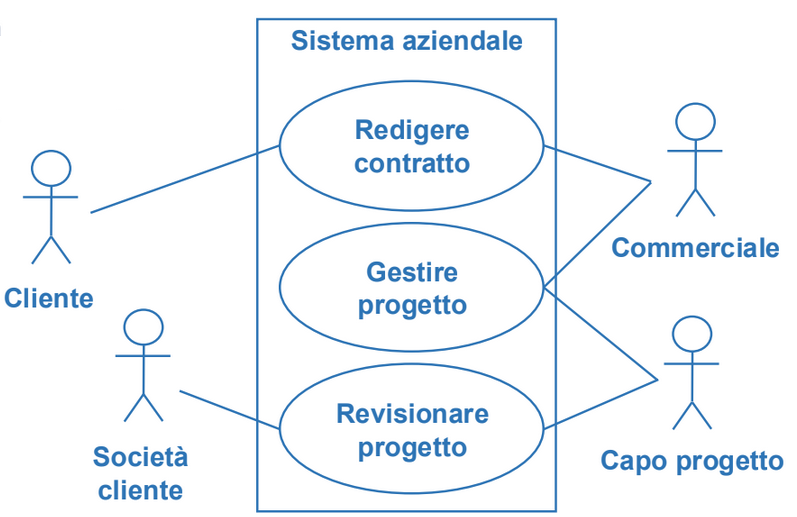
\includegraphics[scale=0.3]{uml_casiuso.png}
\end{center}

\begin{note}
	L'associazione tra attori e casi d'uso è di tipo \textbf{molti a molti} in quanto un attore può essere associato a più casi e un caso a più attori.
\end{note}

\begin{note}
	Un caso può essere \textbf{iniziato} solamente da uno ed un solo attore, detto \textbf{principale} (che può essere il Tempo). Ci sono casi specifici in cui non ci sono attori.
\end{note}

\newpage
\paragraph{Narrativa}
La narrativa descrive il modello dinamico, ovvero gli \textbf{scenari} rilevanti per un caso d'uso dal punto di vista degli attori, compreso il principale. La \textbf{struttura} è la seguente:
\begin{table}[!h]
	\centering
	\begin{tabular}{|c|c|}
		\hline
		\textbf{Nome} & Nome del caso d'uso\\
		\hline
		\textbf{ID} & Identificatore univoco del caso \\
		\hline
		\textbf{Breve descrizione} & $\ldots$\\
		\hline
		\textbf{Attore primario} & Colui che avvia il caso \\
		\hline
		\textbf{Attori secondari} & Tutti gli attori che interagiscono \\
		\hline
		\textbf{Precondizioni} & Ciò che deve valere prima dell'esecuzione\\
		\hline
		\textbf{Sequenza degli eventi principale} & Sequenza di passi \\
		\hline
		\textbf{Postcondizioni} & Ciò che deve valere dopo l'esecuzione \\
		\hline
		\textbf{Sequenze alternative degli eventi} & Errori, ramificazioni e interruzioni\\
		\hline
	\end{tabular}
\end{table}

\paragraph{Scenario}
Uno scenario è un'\textbf{istanza} di un caso d'uso, quindi una sequenza di passi che produce un risultato osservabile da uno o più attori. Portano dalla \textit{precondizione} alla \textit{postcondizione}.
\begin{center}
	
\includegraphics[scale=0.3]{uml_casiuso_scenari.png}
\end{center}

\begin{definition}[Pre e post condizioni]
	Precondizioni e postcondizioni sono \textbf{asserzioni} che devono necessariamente essere vere in uno stato. Si esprimono con \textbf{predicati} e \textbf{formule logiche}. \color{red} Non sono MAI azioni. \color{black}
\end{definition}

\begin{definition}[Flusso di narrativa]
	Per ogni stato $\sigma$ che soddisfa la \textbf{precondizione}, l'esecuzione del caso d'uso a partire da $\sigma$ produce uno stato $\sigma '$ che soddisfa la \textbf{postcondizione}. Questo a meno di imprevisti elencati nella \textit{sequenza alternativa}.
\end{definition}

\paragraph{Sequenza principale}
Indica la sequenza di passi che compongono il caso d'uso. È \textbf{numerata} e ogni passo ha la struttura
\begin{equation*}
	<\text{numero}>.<\text{soggetto}><\text{azione}><\text{complementi}>
\end{equation*}
Il primo passo è detto \textbf{attivazione} ed è compiuto sempre dall'attore principale.

\paragraph{Generalizzazione} È possibile generalizzare gli \textbf{attori}, ad esempio quando c'è bisogno di un unico attore principale (e.g. \textit{professore} e \textit{assistente} sono \textit{ricercatori}), o i \textbf{casi d'uso} (e.g. \textit{card} e \textit{cash} sono \textit{pagamenti}). Bisogna prestare attenzione perché il classificatore specializzato \textbf{eredita} tutte le relazioni di quello padre a meno che non sia esplicitato il contrario.

\begin{definition}[Stereotipo]
	Gli stereotipi sono parole chiave racchiuse tra $<<>>$ che annotano gli elementi di un diagramma, precisandone il significato.
\end{definition}

\paragraph{Inclusione} Un caso d'uso può incorporarne un altro tramite l'\textbf{inclusione}, ovvero la chiamata del primo ha come conseguenza la chiamata del secondo.
\begin{center}
	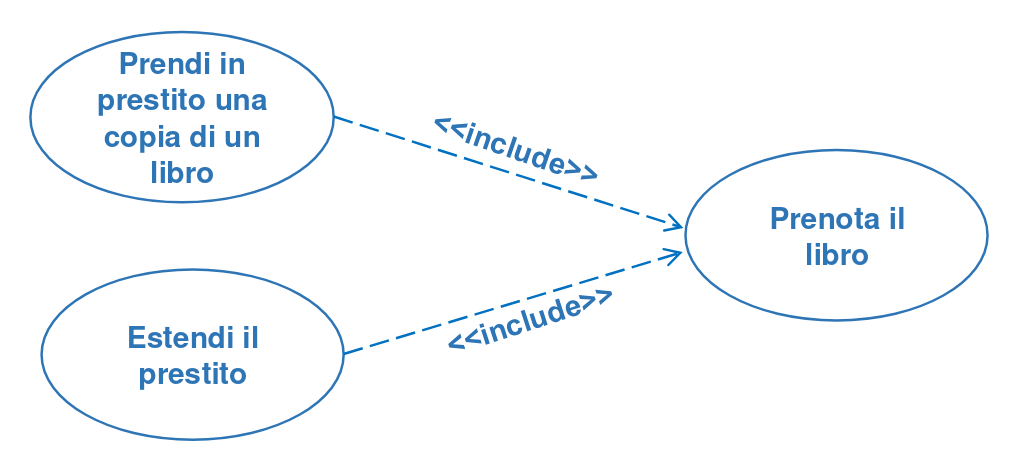
\includegraphics[scale=0.2]{inclusione.png}
\end{center}
Nella narrativa l'inclusione può avvenire in maniera \textit{istanziabile} quando viene avviato da un attore primario o \textit{non istanziabile} quando viene eseguito solo dopo l'inclusione da parte di un altro caso.

\paragraph{Estensione} Quando il primo caso d'uso \textit{può} prevederne un altro, si dice che lo incorpora. Di conseguenza le estensioni sono opzionali e per specificare quando si presentano è possibile usare un \textbf{extension point} con all'interno la condizione che si deve verificare.
\begin{center}
	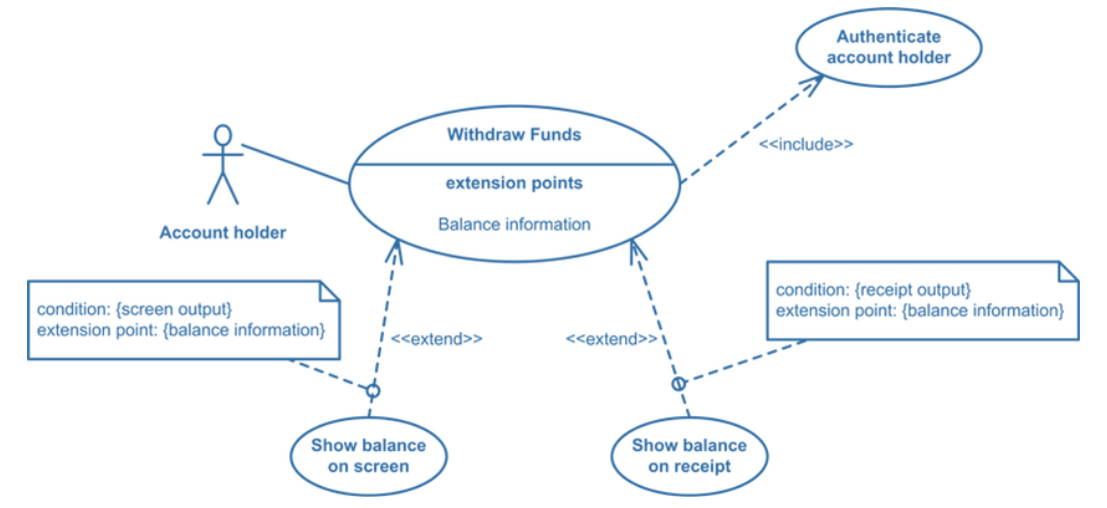
\includegraphics[scale=0.3]{extension.png}
\end{center}

\subsubsection{Classi e oggetti}
Il diagramma delle classi descrive il tipo degli oggetti che fanno parte di un sistema e le relazioni statiche tra di esse. Mostra inoltre le \textbf{proprietà} e le \textbf{operazioni} delle classi. Può essere utilizzato per descrivere il \textit{dominio} o per fare una \textit{progettazione} di dettaglio. 

\begin{definition}[Oggetto]
	Un oggetto è un'identità caratterizzata da un'\textbf{identità}, uno \textbf{stato} (valori e rispettivi attributi) e un \textbf{comportamento} (operazioni che lo definiscono).
\end{definition}
\begin{definition}[Classe]
	Una classe descrive un insieme di oggetti con caratteristiche simili, ovvero dello stesso tipo. Cattura un \textbf{concetto} nel dominio del problema o della realizzazione.
\end{definition}
\noindent In UML la classe contiene:
\begin{itemize}
	\item \textbf{Nome}: maiuscolo singolare
	\item \textbf{Attributi} tipizzati con modificatori di visibilità:
	\begin{itemize}
		\item \textit{Pubblic} \textbf{+} : accessibile ad ogni elemento che può vedere e usare la classe
		\item \textit{Protected} \textbf{\#} : accessibile ad ogni discendente
		\item \textit{Private} \textbf{-} : solo le operazioni della classe vi hanno accesso
		\item \textit{Package} \textbf{\texttildelow} : solo gli elementi dello stesso \textit{package} vi hanno accesso
	\end{itemize}
	\item \textbf{Operazioni} tipizzate
\end{itemize}
\paragraph{Attributi}
La sintassi degli attributi è la seguente:
\begin{equation*}
	\text{visibilità } \textcolor{blue}{nome}: \text{tipo}[\text{\textcolor{orange}{molteplicità}}] = \text{ \textcolor{gray}{valoreIniziale} } \{\text{\textcolor{green}{proprietà}}\}
\end{equation*}
\begin{note}
	La molteplicità $[1]$ può essere omessa.
\end{note}
Degli esempi di \textbf{proprietà} sono \textit{ordered}, \textit{unique} o vincoli in generale (e.g. $\{>0, <10\}$).

\begin{note}
	Quando viene usato per la definizione del dominio, si omettono generalmente \textit{operazioni} e \textit{modificatori di visibilità} e si inseriscono solo gli \textit{attributi} utili ad esso.
\end{note}

\paragraph{Operazioni}
La sintassi delle operazioni è la seguente:
\begin{equation*}
	\text{visibilità } \textcolor{blue}{nome(} \text{\textcolor{orange}{lista parametri}}\textcolor{blue}{)}: \text{tipoRitorno}
\end{equation*}
Dove la lista dei parametri può essere l'\textbf{insieme vuoto} o una \textbf{dichiarazione} di parametro:
\begin{align*}
	\text{\textcolor{orange}{lista parametri}} ::= \emptyset \quad \vert \quad \text{dichiarazione} \\
	\text{dichiarazione} ::= \text{\textcolor{green}{nome}} : \text{tipo} = \text{\textcolor{gray}{default}}
\end{align*}

\begin{note}
	L'unica parte obbligatoria della sintassi è il \textbf{nome}, sia nelle operazioni che in \textit{eventuali} parametri.
\end{note}

\begin{note}
	Attributi e operazioni \textbf{statici}, quindi con ambito di classe, sono \underline{sottolineati}.
\end{note}

\paragraph{Enumerazioni} Le enumerazioni sono usate per specificare un insieme di valori \textbf{prefissati} ovvero tutti i valori che un attributo può assumere.\\
In UML hanno sono \textit{classi} con un nome (il tipo) e l'elenco dei valori. Sono etichettate dallo \textit{stereotipo}
\begin{equation*}
	<<\text{enumeration}>>
\end{equation*}

\subsubsection{Relazioni}
Una relazione rappresenta un legame tra due o più oggetti, di solito istanze di classi diverse.

\begin{table}[!h]
	\centering
	\begin{tabular}{|c|c|}
		\hline
		\textbf{Tra classificatori} & \textbf{Tra oggetti}\\
		\hline
		Associazione & Collegamento \\
		\hline
		Generalizzazione & \textit{(non definita)} \\
		\hline
		Realizzazione & \textit{(non definita)} \\
		\hline
		\multicolumn{2}{|c|}{Dipendenza (d'uso, d'istanza, etc..)}\\
		\hline
	\end{tabular}
\end{table}
\paragraph{Associazione}
Un'associazione è una linea retta con:
\begin{itemize}
	\item \textbf{Nome}, di solito un verbo
	\item \textbf{Ruoli}, di solito sostantivi
	\item \textbf{Verso} di lettura, opzionale
\end{itemize}
Di solito si usa o il \textit{nome} o i \textit{ruoli}, raramente entrambi. \\
È importante anche specificare i \textbf{vincoli di molteplicità}, ovvero il numero di oggetti coinvolti nell'associazione in un dato istante. Si possono definire:
\begin{itemize}
	\item Con un \textbf{numero positivo}
	\item Con il \textbf{simbolo indefinito} (*), ovvero per un qualunque numero $\geq 0$
	\item Indicando gli \textbf{estremi dell'intervallo}, dove quello \textit{inferiore} può essere $\geq 0$ e quello superiore un numero positivo o il simbolo indefinito
\end{itemize}
\begin{example}
	Esempio di molteplicità:
	\begin{center}
		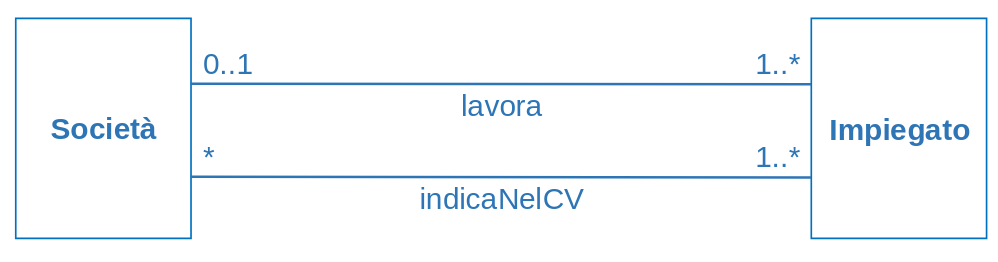
\includegraphics[scale=0.3]{molteplicita.png}
	\end{center}
\end{example}
Un associazione può mettere in relazione un'entità con se stessa, in questo caso è detta \textbf{riflessiva}.\\
Esistono due tipi specifici di associazioni che vengono utilizzati per specificare se un oggetto fa parte o meno di un'altra classe:
\begin{itemize}
	\item \textbf{Aggregazione} ($\Diamond$), poco forte, usata quando la classe "parte" esiste anche senza quella "tutto"
	\item \textbf{Composizione} ($\mathbin{\blacklozenge}$), molto forte, usata quando la classe "parte" non esisterebbe senza quella "tutto". Non ha un nome.
\end{itemize}
\begin{example}
	Esempio di aggregazione e composizione:
	\begin{center}
		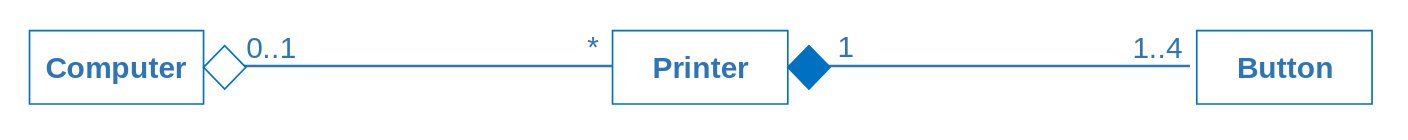
\includegraphics[scale=0.3]{aggr_comp.png}
	\end{center}
\end{example}

\paragraph{Generalizzazione}
È una relazione tra un elemento generico $G$ e uno specializzato $S$, che è consistente con il primo ma contiene più informazione. Per il \textit{principio di sostituzione di Liskov} $S$ può essere sostituito con $G$.
\begin{center}
	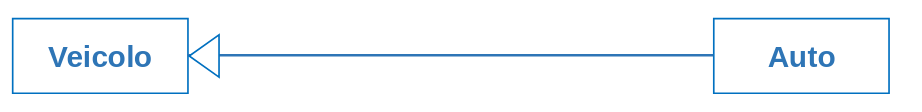
\includegraphics[scale=0.3]{generaliz.png}
\end{center}
Una \textit{superclasse} generalizza le sottoclassi e queste \textbf{ereditano} \textit{attributi}, \textit{operazioni}, \textit{relazioni} e \textit{vincoli}. La sottoclasse può aggiungere caratteristiche e ridefinire determinate operazioni.
\begin{center}
	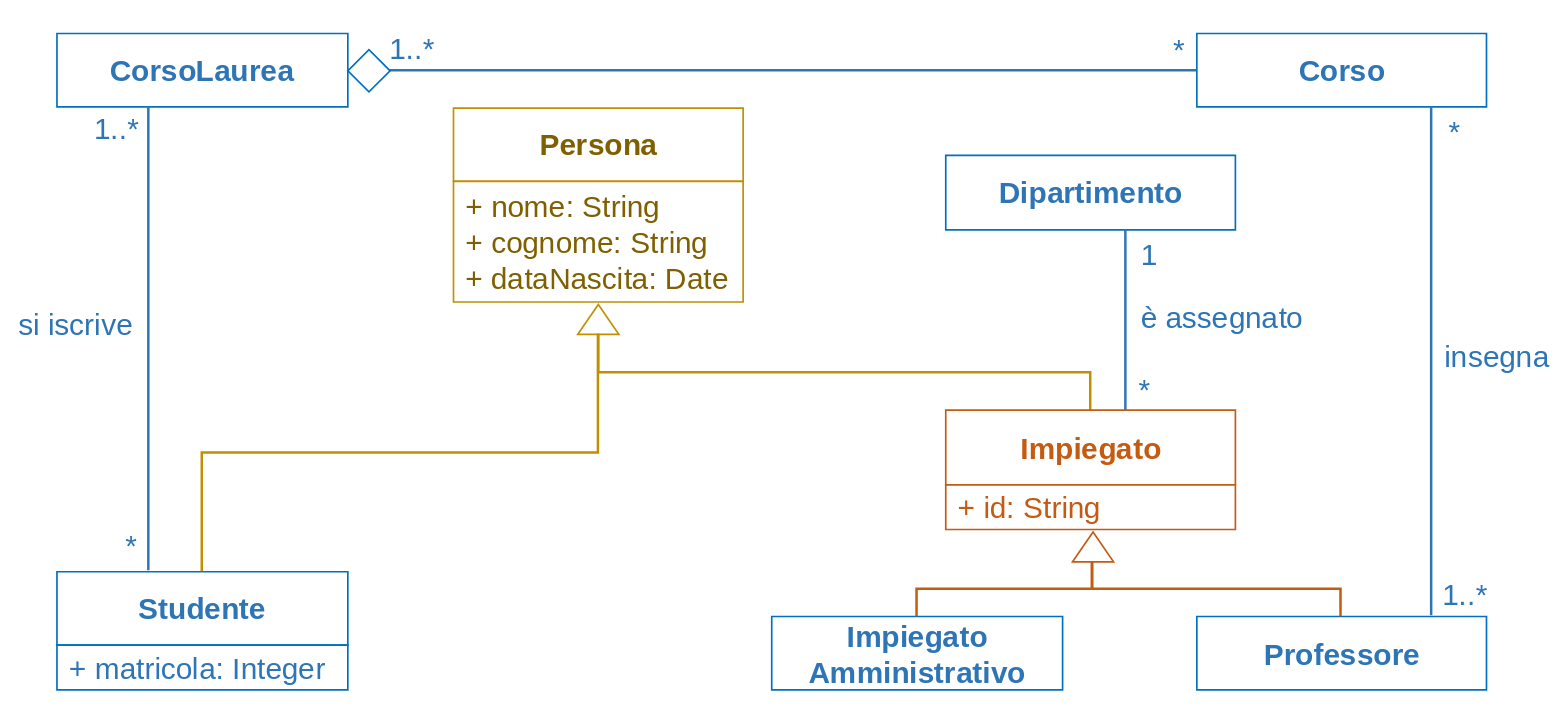
\includegraphics[scale=0.25]{generaliz_ex.png}
\end{center}

\begin{definition}[Classe astratta]
	Nell'ambito della generalizzazione, quando una classe esiste puramente per essere poi estesa e specializzata, viene definita \textbf{astratta}. In questo caso o si usa il nome in corsivo o si indica 
	\begin{equation*}
		\{\text{abstract}\}
	\end{equation*}
\end{definition}

\begin{definition}[Interfaccia]
	Un'interfaccia è un'entità che contiene solamente il comportamento ma nessuno stato. Viene indicata dallo stereotipo
	\begin{equation*}
		<<\text{interface}>>
	\end{equation*}
\end{definition}

\paragraph{Dipendenza}
Una dipendenza è una relazione tra una classe \textbf{cliente} e una \textbf{fornitore}, dove il primo dipende dal secondo e una modifica nel secondo influenza il primo. Viene indicata da una linea tratteggiata con uno dei seguenti stereotipi a seconda del caso
\begin{equation*}
	<<\text{use}>> \qquad <<\text{create}>>
\end{equation*}

\subsubsection{Classi di analisi}
Le classi di analisi corrispondo a concetti concreti del \textit{dominio}, e.g. il contenuto del glossario. Viene spesso raffinata in una o più classi di \textit{progettazione}. Il loro compito è quello di \textbf{astrarre} un elemento del dominio. Generalmente devono seguire le seguenti caratteristiche:
\begin{itemize}
	\item Numero ridotto di funzionalità
	\item Evitare classi \textit{onnipotenti}
	\item Evitare funzioni travestite da classi
	\item Evitare gerarchie di ereditarietà $\geq 3$
\end{itemize}
Esistono principalmente due approcci per identificare le classi di analisi:
\begin{itemize}
	\item \textbf{Data-driven}: si identificano i dati del sistema e si dividono in classi, tipico per la fase di analisi
	\item \textbf{Responsibility-driven}: si identificano le responsabilità e si dividono in classi, tipico per la fase di progettazione
\end{itemize}
\paragraph{Analisi nome-verbo}
Una tecnica per eseguire l'identificazione dove ogni \textbf{sostantivo} corrisponde ad una \textit{classe} o \textit{attributo} mentre ogni \textbf{verbo} ad un'operazione.\\
Consiste in:
\begin{enumerate}
	\item Individuazione delle classi
	\item Assegnazione di attributi e responsabilità
	\item Individuazione delle relazioni
\end{enumerate}
Le problematiche principali sono i sinonimi che portano a classi \textbf{inutili} e le classi \textbf{nascoste} perché implicite nel dominio.

\subsubsection{Diagramma degli oggetti}
Un oggetto si rappresenta con il \textbf{nome}, la \textbf{classe} che istanzia, \underline{sottolineati} e la lista degli \textbf{attributi} (nome, tipo e valore).
\paragraph{Collegamento} Un collegamento istanzia un'associazione nel diagramma delle classi collegando due o più oggetti. Non ha nome, ha sempre molteplicità $1:1$ e può includere i ruoli

\begin{figure}[!h]
	\centering
	\begin{minipage}[b]{0.5\textwidth}
		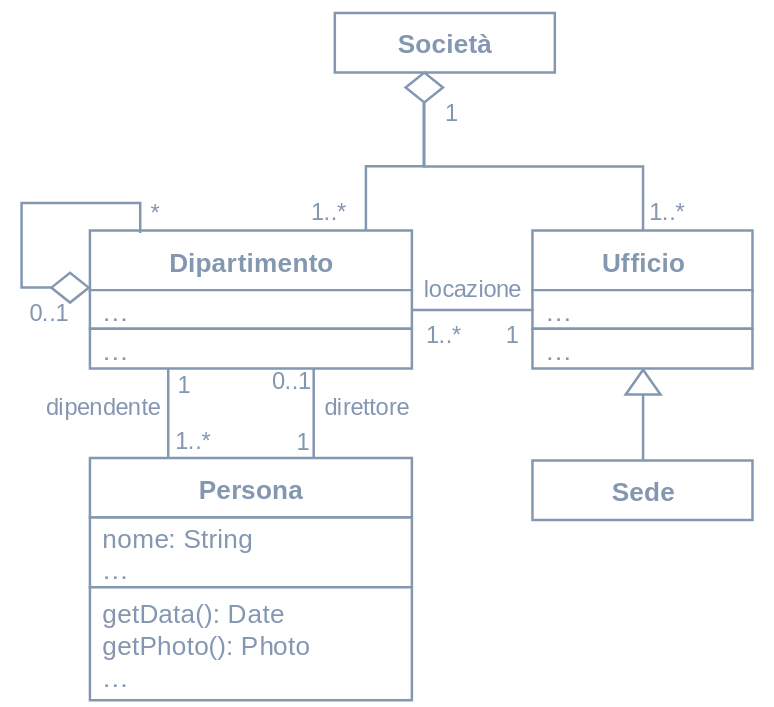
\includegraphics[width=\textwidth]{diag_class.png}
		\caption{Diagramma delle classi}
	\end{minipage}
	\hfill
	\begin{minipage}[b]{0.4\textwidth}
		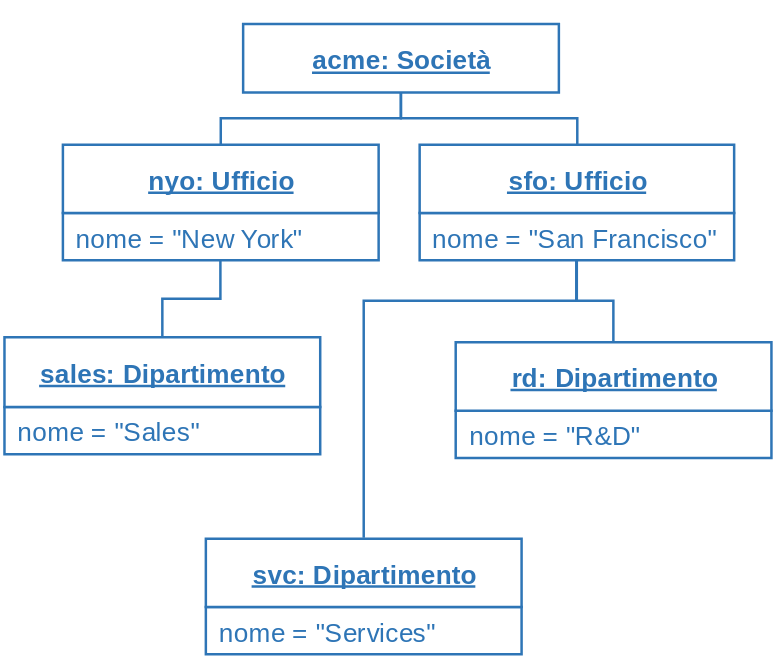
\includegraphics[width=\textwidth]{diag_obj.png}
		\caption{Diagramma degli oggetti}
	\end{minipage}
\end{figure}

\subsubsection{Diagramma delle attività}
Il diagramma delle attività modella un \textbf{workflow} e descrive come \textbf{coordinare} un insieme di \textbf{azioni}, quali \textit{sequenze}, \textit{scelte}, \textit{iterazioni} e \textit{concorrenza}.
Nello specifico modella un'attività in cui sono coinvolte una o più entità.\\
In UML è contenuta in un rettangolo dagli angoli smussati e ha un nome.
\begin{center}
	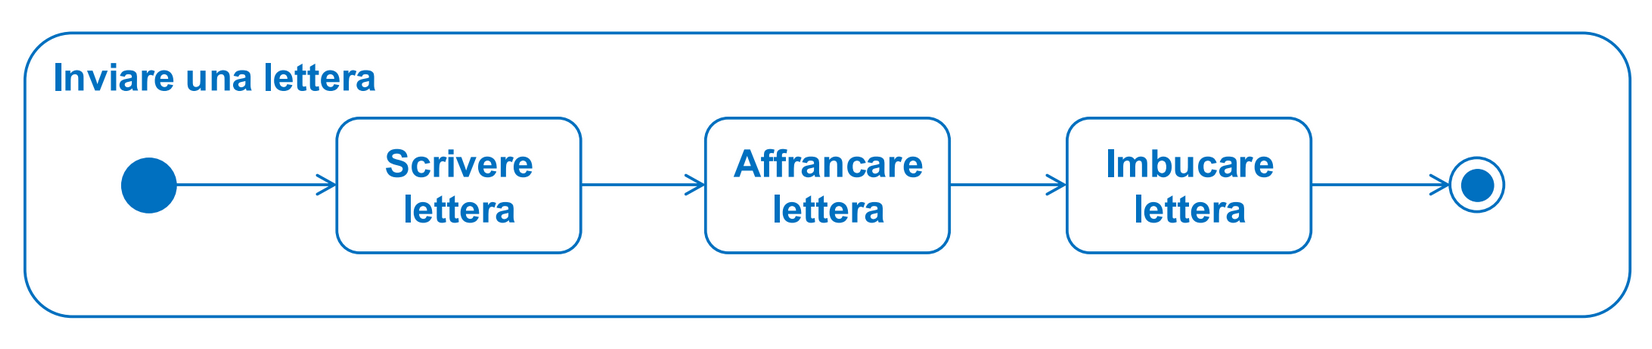
\includegraphics[scale=0.2]{activity.png}
\end{center}
Il contenuto dell'attività è un \textbf{grafo diretto}, dove i \textbf{nodi} rappresentano le componenti dell'attività (azioni e nodi di controllo quali inizio e fine) mentre gli \textbf{archi} rappresentano il \textbf{control flow}, ovvero i possibili path di esecuzione.

\paragraph{Azioni} Le azioni sono rettangoli con gli angoli smussati che contengono il nome che è sempre un \textbf{verbo}. Sono \textbf{atomiche} e non interrompibili.\\
Ogni azione ha solo un arco entrante ed uno uscente e quest'ultimo viene attraversato ad azione terminata, simulando il passaggio di un \textbf{token} che permette l'esecuzione.

\paragraph{Nodi di controllo} Sono nodi che alterano il control flow. Possono essere:
\begin{itemize}
	\item \textbf{Decisione} e \textbf{fusione}: sono rappresentati da rombi, nel primo caso con condizioni che devono coprire tutti i possibili casi ($X \lor Y \lor \ldots \lor Z = \text{true}$) e che portano a rami differenti. È possibile utilizzare la clausola \textit{$[\text{else}]$}. Non è obbligatorio che ci sia un nodo di fusione corrispondente.
	\begin{center}
		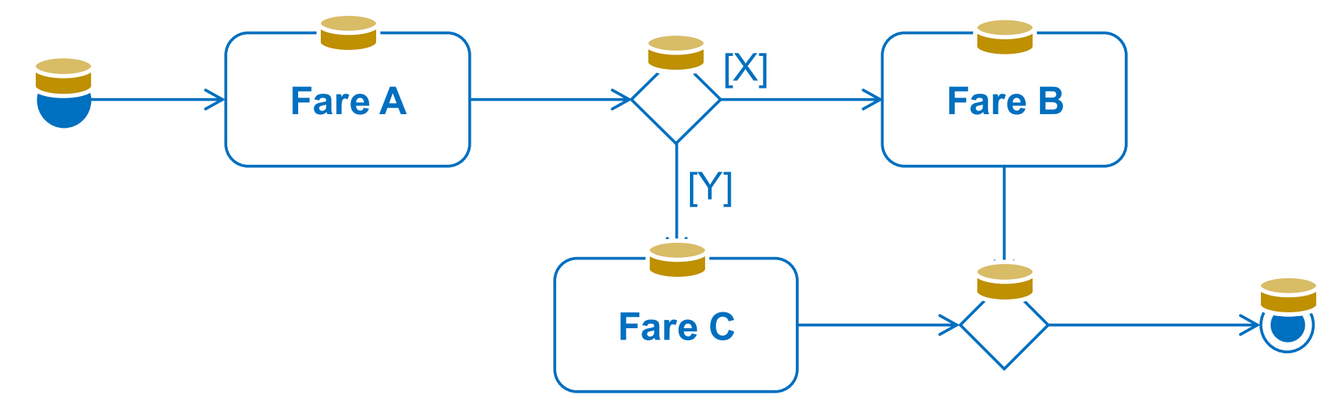
\includegraphics[scale=0.2]{decision_fusion.png}
	\end{center}
	\item \textbf{Fork} e \textbf{join}: la fork moltiplica i token e ne restituisce uno per ogni ramo uscente, al contrario la join (non ne serve per forza una per ogni fork), attende un token da ogni ramo, li consuma tutti e ne restituisce uno.
	\begin{center}
		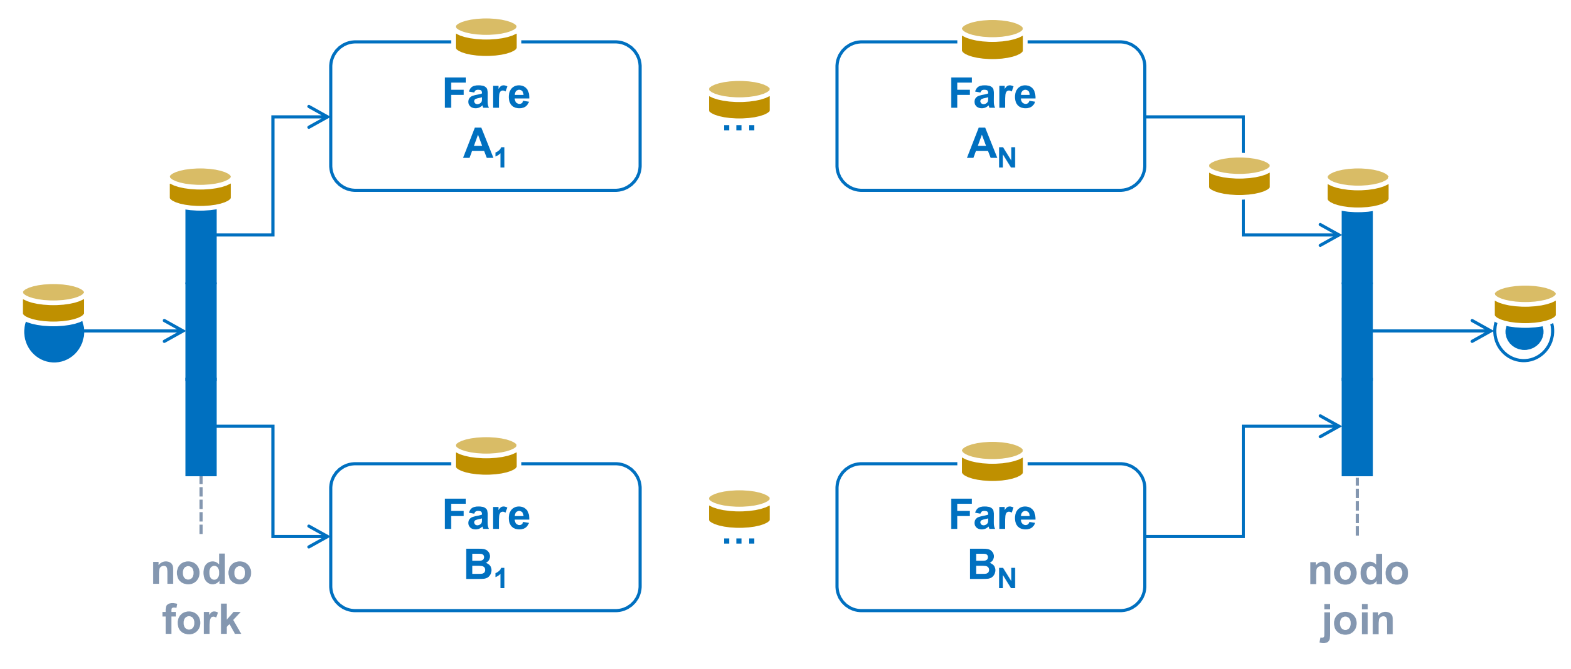
\includegraphics[scale=0.2]{fork_join.png}
	\end{center}
	\item \textbf{Fine attività} e \textbf{fine flusso}: gli unici nodi che possono avere più archi entranti. Il primo, appena riceve un token, termina l'intera attività mentre il secondo termina solo il flusso corrispondente.
	\begin{center}
		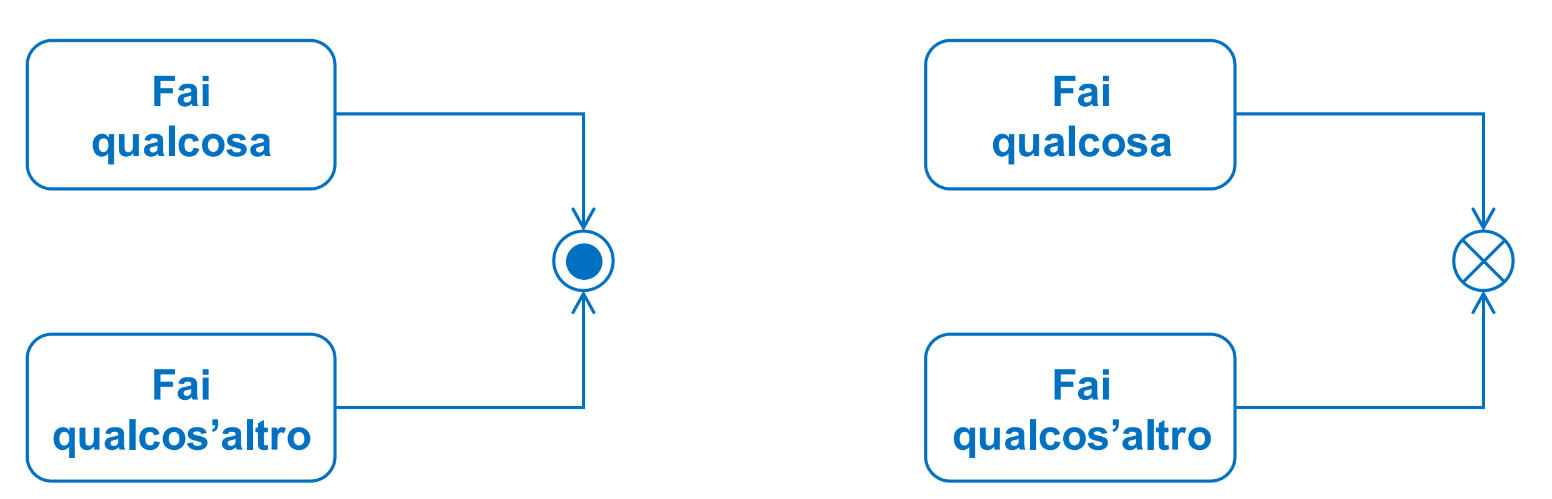
\includegraphics[scale=0.2]{end_node.png}
	\end{center}
	\newpage
	\item \textbf{Segnali} ed \textbf{eventi}: possono inviare un \textbf{segnale asincrono}, riceverlo o accettare un \textbf{evento temporale} (assoluto o relativo)
	\begin{figure}[!h]
		\centering
		\begin{minipage}[b]{0.2\textwidth}
			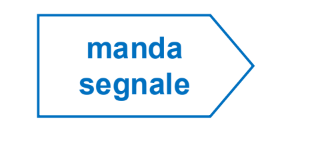
\includegraphics[width=\textwidth]{send_signal.png}
			\caption*{Invio}
		\end{minipage}
		\hspace{0.1\textwidth}
		\begin{minipage}[b]{0.2\textwidth}
			
\includegraphics[width=\textwidth]{accept_signal.png}
			\caption*{Accettazione}
		\end{minipage}
		\hspace{0.1\textwidth}
		\begin{minipage}[b]{0.2\textwidth}
			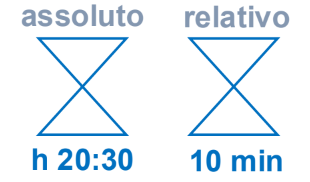
\includegraphics[width=\textwidth]{time_signal.png}
			\caption*{Evento temporale}
		\end{minipage}
	\end{figure}
	I nodi di accettazione non hanno bisogno di archi entranti: se non c'è si genera un token quando si verifica l'evento, altrimenti si attende prima di passarlo al nodo successivo.
\end{itemize}

\begin{note}[Fork e merge]
	È possibile eseguire una \textit{fork} e poi una \textit{merge} invece della join, ma questo vorrà dire che le operazioni dopo saranno eseguite più volte.
\end{note}

\begin{note}[Azioni vs eventi]
	Un'\textbf{azione} si usa quando è effettuata da una o più entità che stiamo descrivendo mentre un \textbf{evento} riguarda quelle esterne.
\end{note}

\paragraph{Sotto attività}
Un diagramma può contenere un riferimento ad un'attività secondaria e viene indicato con $\pitchfork$.

\paragraph{Partizionamento} Sono divisioni dell'attività che permettono di assegnare le responsabilità, spesso usate ad esempio in combinazione con la divisione delle unità operative di un modello business.
\begin{center}
	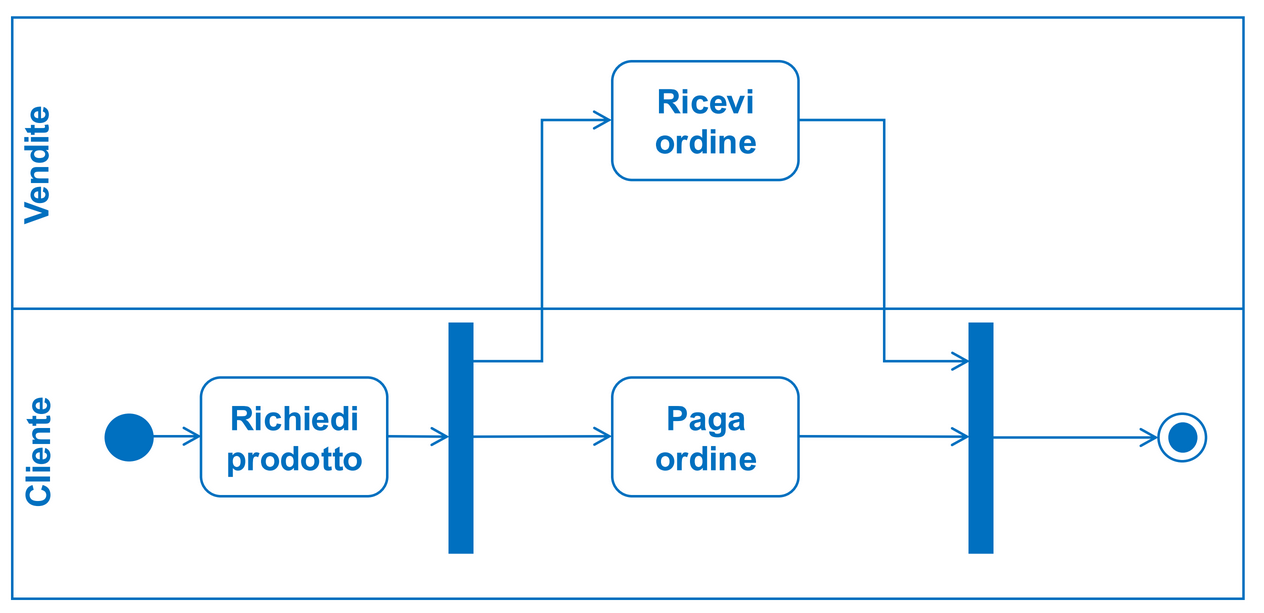
\includegraphics[scale=0.3]{partition.png}
\end{center}

\subsubsection{Comportamenti}
Il comportamento di una classe viene descritto da un \textbf{grafo stati-transizioni}. Questo contiene gli \textbf{stati} significativi di un oggetto durante la sua vita e come questo può \textbf{transire} (in seguito ad eventi) tra di essi.
\end{document}
